
\documentclass[12pt, twoside,openany]{book}
%%%%%%%% Preamble %%%%%%%%%%%%
\title{Optimización de Tiempos de Espera en Intersecciones mediante Aprendizaje por Refuerzo Profundo y Simulación}
\usepackage[utf8]{inputenc} % File coding uses utf8
\usepackage{amsmath} % Extra commands for math
\usepackage{amssymb} % Math symbols 
\usepackage{graphicx} % Include images in LaTeX
\usepackage{color} % Coloring text
\usepackage{enumerate}
\usepackage{float} % Allow you to use [H] specifier to force the position of the images 
\usepackage{capt-of} % Defines a command \captionof for putting a caption to something that’s not a float.
\usepackage{sidecap} % Defines environments called SCfigure and SCtable (analogous to figure and table) to typeset captions sideways
	\sidecaptionvpos{figure}{c} % Alignment
\usepackage{caption} % to customize the captions in floating environments like figure and table
\usepackage{commath} % Mathematics typesetting support
\usepackage{cancel} % Place lines through maths formulae
\usepackage{anysize} % to set up document margins
%\marginsize{2cm}{2cm}{2cm}{2cm} % Left, right, up, down
%\usepackage[top=2cm,bottom=4cm,left=1.5cm,right=3cm,asymmetric]{geometry}
\usepackage{appendix} %Extra control of appendices
\usepackage{tocbibind}
\usepackage{anyfontsize}
\newcommand\mymaintitlesize{\fontsize{16pt}{19.2pt}\selectfont}
\newcommand\mysubtitlesize{\fontsize{14pt}{16.8pt}\selectfont}


%EXTRA PACKAGES
\usepackage{booktabs}
\usepackage{multirow}
\usepackage{glossaries}
\usepackage[linesnumbered,ruled,vlined]{algorithm2e}
\usepackage{multirow}
\usepackage{enumerate}
\usepackage{changepage}
\usepackage{alltt}
\usepackage{listings}
\usepackage{lmodern}
\usepackage{caption}
\usepackage{subcaption}
\usepackage{hyperref}
\usepackage{xurl}
\hypersetup{
    colorlinks,
    citecolor=blue,
    filecolor=black,
    linkcolor=black,
    urlcolor=black
}
\urlstyle{same}
\pdfstringdefDisableCommands{\let\centering\relax}
\usepackage{setspace}
\setstretch{1.5}
\usepackage{listings}
\usepackage{color}
\lstloadlanguages{C,C++,csh,Java}

\definecolor{red}{rgb}{0.6,0,0} 
\definecolor{blue}{rgb}{0,0,0.6}
\definecolor{green}{rgb}{0,0.8,0}
\definecolor{cyan}{rgb}{0.0,0.6,0.6}

\lstset{
language=csh,
basicstyle=\footnotesize\ttfamily,
numbers=left,
numberstyle=\tiny,
numbersep=5pt,
tabsize=2,
extendedchars=true,
breaklines=true,
frame=b,
stringstyle=\color{blue}\ttfamily,
showspaces=false,
showtabs=false,
xleftmargin=17pt,
framexleftmargin=17pt,
framexrightmargin=5pt,
framexbottommargin=4pt,
commentstyle=\color{green},
morecomment=[l]{//}, %use comment-line-style!
morecomment=[s]{/*}{*/}, %for multiline comments
showstringspaces=false,
morekeywords={ abstract, event, new, struct,
as, explicit, null, switch,
base, extern, object, this,
bool, false, operator, throw,
break, finally, out, true,
byte, fixed, override, try,
case, float, params, typeof,
catch, for, private, uint,
char, foreach, protected, ulong,
checked, goto, public, unchecked,
class, if, readonly, unsafe,
const, implicit, ref, ushort,
continue, in, return, using,
decimal, int, sbyte, virtual,
default, interface, sealed, volatile,
delegate, internal, short, void,
do, is, sizeof, while,
double, lock, stackalloc,
else, long, static,
enum, namespace, string},
keywordstyle=\color{cyan},
identifierstyle=\color{red},
backgroundcolor=\color{white},
}

\lstdefinestyle{sharpc}{language=[Sharp]C, frame=lr, rulecolor=\color{blue!80!black}}

% Reset page margins properly for doublesided pages
\setlength{\marginparwidth}{0pt}
\setlength{\marginparsep}{0pt}
\setlength{\oddsidemargin}{0.125in}
\setlength{\evensidemargin}{0.125in}
\setlength{\textwidth}{6.375in}
\setlength{\emergencystretch}{2em}
\raggedbottom


%%% Theorem-like environments %%%%%%%%%%%%%%%%%%%%%%%%%%%%%%%%%%%%%%%%%%%%%%%%%%
%%\usepackage{mathtools}

\newtheorem{theorem}{Theorem}
\newtheorem{corollary}{Corollary}
\newtheorem{lemma}{Lemma}
\newtheorem{proposition}{Proposition}
\newtheorem{conjecture}{Conjecture}
\newtheorem{definition}{Definition}
\newtheorem{remark}{Remark}
\newtheorem{example}{Example}

%%%%%%%%%%%%%%%%%%%%%%%%%%%%%%%%%%%%%%%%%%%%%%%%%%%%%%%%%%%%%%%%%%%%%%%%%%%%%%%%

%%% Put your local definitions here %%%%%%%%%%%%%%%%%%%%%%%%%%%%%%%%%%%%%%%%%%%%
% For example,
\newcommand{\R}{\mathbb{R}}


% Header and Footer
\usepackage{fancyhdr} 
\pagestyle{empty}
\renewcommand{\headrulewidth}{0pt}
\renewcommand{\footrulewidth}{0pt}
\fancypagestyle{firststyle}
{
   \fancyhf{}
   \renewcommand{\headrulewidth}{0pt}
   \renewcommand{\footrulewidth}{0pt}
}

\usepackage{listings} % To use source code
\definecolor{dkgreen}{rgb}{0,0.6,0} % Color for using code
\definecolor{gray}{rgb}{0.5,0.5,0.5} 
% Language to use

\title{Optimización de Tiempos de Espera en Intersecciones mediante Aprendizaje por Refuerzo Profundo y Simulación}


\newglossaryentry{drl}
{
        name=DRL,
        description={Deep Reinforcement Learning (Aprendizaje por Refuerzo Profundo). Rama del aprendizaje automático que combina redes neuronales profundas con algoritmos de aprendizaje por refuerzo}
}

\newglossaryentry{ppo}
{
        name=PPO,
        description={Proximal Policy Optimization. Algoritmo de gradiente de política utilizado en aprendizaje por refuerzo que busca mejorar la estabilidad del entrenamiento limitando el tamaño de las actualizaciones de la política}
}

\newglossaryentry{sumo}
{
        name=SUMO,
        description={Simulation of Urban MObility. Paquete de simulación de tráfico multimodal, microscópico, de código abierto y continuo}
}

\newglossaryentry{throughput}
{
        name=Throughput,
        description={Caudal vehicular o flujo vehicular efectivo. Medida de la cantidad de vehículos que logran atravesar una intersección o segmento vial en un periodo de tiempo determinado}
}

\newglossaryentry{rl}
{
        name=RL,
        description={Reinforcement Learning (Aprendizaje por Refuerzo). Paradigma de aprendizaje automático donde un agente aprende a tomar decisiones mediante la interacción con un entorno y la recepción de recompensas}
}

\newglossaryentry{mdp}
{
        name=MDP,
        description={Markov Decision Process (Proceso de Decisión de Markov). Marco matemático para modelar la toma de decisiones en situaciones donde los resultados son en parte aleatorios y en parte bajo el control de un tomador de decisiones}
}

%%%%%%%% Preamble ends %%%%%%%%%%%%

\begin{document}
\linespread{1.25}
%%%%%%%%%%%%%%%%%%%%%%%%%%%%%%%% Cover Page %%%%%%%%%%%%%%%%%%%%%%%%%%%%%%%%%%%%%%%%%%%

\thispagestyle{empty}
\begin{center}
\begin{figure}
    \centering
    \includegraphics[scale = 0.9828]{images/logo_universidad.png}
\end{figure}
{\fontsize{18pt}{21.6pt}\selectfont \textbf{UNIVERSIDAD DE INVESTIGACIÓN DE TECNOLOGÍA EXPERIMENTAL YACHAY}}\\
\vspace*{0.75cm}
{\mysubtitlesize{\textbf{Escuela de Ciencias Matemáticas y Computacionales}}}\\
\vspace*{1.75cm}
{\mymaintitlesize{\textbf{TÍTULO: Optimización de Tiempos de Espera en Intersecciones mediante Aprendizaje por Refuerzo Profundo y Simulación}}\\
\vspace*{0.75cm}
Trabajo de titulación presentado como requisito para la obtención del título de Magíster en Inteligencia Artificial}\\
\vspace*{1.75cm}
{\mysubtitlesize{\textbf{Autor:}\\
\vspace*{0.5cm}
Bryan Andres Ortega Llanos\\
\vspace*{0.75cm}
\textbf{Tutor:}\\
\vspace*{0.5cm}
PhD. Tito Rolando Armas Andrade\\
\vspace*{1.75cm}
Urcuquí, marzo de 2026}}

\end{center}
\pagenumbering{gobble}
%%%%%%%%%%%%%%%%%%%% Cover page ends %%%%%%%%%%%%%%%%%%%%%%%%%%%%%%%%


\clearpage
\pagenumbering{roman}

\chapter*{\centering Autoría}
\label{chap:autoria}

Yo, \textbf{Bryan Andres Ortega Llanos}, con cédula de identidad 1003979786, declaro que las ideas, juicios, valoraciones, interpretaciones, consultas bibliográficas, definiciones y conceptualizaciones expuestas en el presente trabajo; así cómo, los procedimientos y herramientas utilizadas en la investigación, son de absoluta responsabilidad de el/la autor/a del trabajo de titulación. Así mismo, me acojo a los reglamentos internos de la Universidad de Investigación de Tecnología Experimental Yachay.

\vspace{0.6cm}

\noindent Urcuquí, 1 de marzo de 2026.

\vspace{2.5cm}

\begin{center}
    \rule[0mm]{60mm}{0.1mm} \\
    {Bryan Andres Ortega Llanos}\\
    CI: 1003979786
\end{center}

\thispagestyle{empty} % para que no se numere esta pagina	


\chapter*{\centering Autorización de publicación}
\label{chap:autorizacion}
Yo, \textbf{Bryan Andres Ortega Llanos}, con cédula de identidad 1003979786, cedo a la Universidad de Investigación de Tecnología Experimental Yachay, los derechos de publicación de la presente obra, sin que deba haber un reconocimiento económico por este concepto. Declaro además que el texto del presente trabajo de titulación no podrá ser cedido a ninguna empresa editorial para su publicación u otros fines, sin contar previamente con la autorización escrita de la Universidad.

\vspace{0.6cm}

\noindent Asimismo, autorizo a la Universidad que realice la digitalización y publicación de este trabajo de integración curricular en el repositorio virtual, de conformidad a lo dispuesto en el Art. 144 de la Ley Orgánica de Educación 

\vspace{0.6cm}

\noindent Urcuquí, Noviembre 2025.

\vspace{2.5cm}

\begin{center}
    \rule[0mm]{60mm}{0.1mm} \\
    {Bryan Andres Ortega Llanos}\\
    CI: 1003979786
\end{center}

\thispagestyle{empty} % para que no se numere esta pagina

\chapter{\centering Dedicatoria}
\label{chap:dedication}
\vspace*{3cm}
\begin{center}
\textit{A mi esposa Naty, el amor de mi vida y mi apoyo incondicional.}

\textit{A mis padres, quienes sembraron en mí el deseo de superación.}

\textit{A mis hermanos Jorge y Dylan, y a mi querida abuelita Merceditas.}

\textit{Este logro es de todos ustedes.}
\end{center}

\chapter{\centering Agradecimientos}
\label{chap:acknowledgments}
Quiero expresar mi sincero agradecimiento a la \textbf{Universidad Yachay Tech} por abrirme las puertas de esta maestría y brindarme las herramientas para crecer profesionalmente.

A mi tutor, \textbf{PhD. Tito Armas}, por su guía, paciencia y valiosos consejos que orientaron el desarrollo de esta investigación. A mis profesores, por compartir su conocimiento y exigirme dar lo mejor de mí.

Un agradecimiento especial a mi familia, pilar fundamental de este sueño:

A mi esposa \textbf{Naty}, por estar siempre a mi lado, por las noches de desvelo acompañándome y por cuidarme con tanto cariño, incluso pasándome un plato de comida mientras atendía clases.

A mis \textbf{padres}, por el inmenso esfuerzo de financiar mis estudios y confiar en mi capacidad. Esta beca y este título son mi forma de honrar su sacrificio.

A mi hermano \textbf{Jorge}, por ser más que un hermano, un gran compañero de clases y estudio. A mi hermano \textbf{Dylan}, por cubrirme la espalda en el trabajo siempre que lo necesité.

A mi abuelita \textbf{Merceditas}, por sus visitas llenas de dulzura y por estar siempre pendiente de mí.


\chapter{\centering Resumen}
\label{chap:resumen}
Este trabajo presenta el desarrollo de un sistema de control semafórico adaptativo basado en \textbf{Deep Reinforcement Learning (DRL)} utilizando el algoritmo \textbf{Proximal Policy Optimization (PPO)} integrado con el simulador microscópico de tráfico \textbf{SUMO}. El objetivo principal es reducir la congestión urbana mediante la optimización dinámica de tiempos semafóricos en una intersección crítica.

El agente aprende a manejar condiciones de tráfico altamente variables gracias a una función de recompensa diseñada para balancear eficiencia y estabilidad, incorporando penalizaciones por colas, desequilibrio direccional y cambios excesivos de fase. El entrenamiento se realizó bajo un perfil de tráfico dinámico de 60 minutos con múltiples picos de demanda.

Los resultados muestran una \textbf{reducción aproximada del 60\% en la longitud promedio de colas} y un \textbf{incremento del 4.5\% en el flujo vehicular efectivo (throughput)} respecto a un controlador de tiempo fijo. Estos resultados demuestran la efectividad del enfoque DRL + SUMO para mejorar la movilidad urbana. Finalmente, se discuten las limitaciones actuales y se proponen líneas de trabajo futuro, incluyendo control multiagente y percepción mediante visión por computador.

\vspace{1em}
\noindent \textbf{Palabras clave:} semáforos inteligentes, aprendizaje por refuerzo, PPO, SUMO, tráfico urbano.

\chapter{\centering Abstract}
\label{chap:abstract}
This thesis presents the development of an adaptive traffic signal controller based on \textbf{Deep Reinforcement Learning (DRL)} using the \textbf{Proximal Policy Optimization (PPO)} algorithm integrated with the microscopic traffic simulator \textbf{SUMO}. The main objective is to reduce urban congestion by dynamically optimizing signal timings in a high-demand intersection.

The agent learns to manage highly variable traffic conditions through a reward function designed to balance efficiency and stability, incorporating penalties for queue length, directional imbalance, and frequent phase switching. Training was conducted under a dynamic 60-minute traffic profile with several demand peaks.

Results show an \textbf{approximate 60\% reduction in average queue length} and a \textbf{4.5\% increase in throughput} compared to a fixed-time controller. These findings demonstrate the effectiveness of combining DRL and SUMO to improve urban mobility. Limitations and future work directions are discussed, including multi-agent control and perception via computer vision.

\vspace{1em}
\noindent \textbf{Keywords:} intelligent traffic lights, reinforcement learning, PPO, SUMO, urban mobility.

\tableofcontents 
\printglossaries
\listoftables
\listoffigures




\mainmatter

\newpage

\chapter{Introducción}
\label{chap:intro}
\section{Contexto del problema}
El crecimiento urbano y el aumento del parque automotor han provocado que las intersecciones semaforizadas se conviertan en puntos críticos de congestión. Los semáforos tradicionales, basados en ciclos fijos, no consideran la variabilidad temporal del flujo vehicular ni las diferencias entre direcciones. En ciudades intermedias, donde la demanda presenta picos súbitos y asimétricos, los controladores fijos generan colas extensas, tiempos de espera elevados y un uso ineficiente del espacio vial.

\section{Motivación}
La gestión adaptativa del tráfico representa una oportunidad para reducir de manera significativa la congestión mediante el uso de técnicas modernas de inteligencia artificial. Los avances en \textbf{Deep Reinforcement Learning (DRL)} y la capacidad de simular escenarios realistas con \textbf{SUMO} permiten entrenar agentes capaces de aprender políticas óptimas para la asignación de tiempos semafóricos, respondiendo de forma dinámica a cambios en la demanda. Esta tesis busca aplicar dichas técnicas para mejorar la movilidad urbana en un cruce representativo de la ciudad.

\section{Planteamiento del problema}
Los sistemas semafóricos de tiempo fijo son ineficientes cuando la demanda vehicular no es uniforme ni estable. En situaciones de alto tráfico, estos sistemas mantienen fases verdes incluso cuando no existen vehículos, mientras otras aproximaciones acumulan colas. El problema a resolver es: \textbf{¿cómo optimizar los tiempos semafóricos de una intersección utilizando DRL para minimizar la formación de colas y mejorar el flujo vehicular bajo condiciones dinámicas y variables?}

\section{Objetivo general}
Desarrollar un sistema de control semafórico adaptativo basado en \textbf{Proximal Policy Optimization (PPO)}, integrado con SUMO, capaz de reducir colas, mejorar el throughput (caudal vehicular) y adaptarse a variaciones en la demanda vehicular.

\section{Objetivos específicos}
\begin{itemize}
    \item Diseñar e implementar un entorno de simulación de tráfico en SUMO para un cruce urbano representativo.
    \item Definir y configurar un agente DRL basado en PPO para el control de fases semafóricas.
    \item Construir una función de recompensa que guíe al agente hacia políticas eficientes y estables.
    \item Entrenar el agente bajo diferentes perfiles de tráfico dinámico.
    \item Evaluar el desempeño del agente comparándolo con un controlador de tiempo fijo.
\end{itemize}

\section{Justificación}
El impacto de la congestión vehicular trasciende la mera incomodidad de los conductores; se manifiesta en pérdidas económicas significativas, incremento en el consumo de combustibles fósiles y un aumento preocupante en las emisiones de gases de efecto invernadero. En ciudades en desarrollo, la infraestructura vial rígida no puede expandirse al mismo ritmo que el parque automotor. Por tanto, la optimización del uso de la infraestructura existente se vuelve imperativa.

Implementar estrategias inteligentes basadas en \textbf{Deep Reinforcement Learning (DRL)} permite transitar de un paradigma reactivo y estático a uno proactivo y dinámico. A diferencia de los sistemas tradicionales que requieren costosas recalibraciones manuales, un agente DRL aprende y evoluciona con el tráfico. Además, la integración con simuladores de código abierto y estandarizados como \textbf{SUMO} garantiza no solo la viabilidad técnica y económica del proyecto, sino también su reproducibilidad y rigor científico, abriendo la puerta a futuras implementaciones en hardware real a bajo costo.

\section{Alcance y limitaciones}
\textbf{Alcance:}
\begin{itemize}
    \item Se estudia una intersección específica con alto flujo vehicular.
    \item El agente controla únicamente el ciclo semafórico.
    \item Las pruebas se realizan en un entorno simulado.
\end{itemize}

\textbf{Limitaciones:}
\begin{itemize}
    \item No se implementa el sistema en infraestructura real.
    \item El modelo no considera peatones ni transporte público.
    \item La percepción del entorno se basa en datos simulados (no cámaras reales).
\end{itemize}


\chapter{Marco Teórico}
\label{chap:theory}
\section{Conceptos de Tránsito Vehicular}
El análisis del tráfico vehicular se fundamenta en la teoría del flujo vehicular, la cual describe la interacción entre vehículos, conductores e infraestructura. Las variables macroscópicas fundamentales son:

\textbf{Flujo ($q$):} Se define como la tasa a la cual los vehículos pasan por un punto específico de la vía durante un intervalo de tiempo. Se expresa comúnmente en vehículos por hora (veh/h) \cite{survey_prajapati2024,survey_haydari2022}.
\begin{equation}
    q = \frac{N}{T}
\end{equation}
Donde $N$ es el número de vehículos que pasan por el punto y $T$ es el intervalo de tiempo de observación.

\textbf{Densidad ($k$):} Representa el número de vehículos ocupando un segmento de longitud unitaria de la vía en un instante dado. Se expresa en vehículos por kilómetro (veh/km) \cite{survey_haydari2022}.

\textbf{Velocidad media espacial ($v_s$):} Es la media armónica de las velocidades de los vehículos que pasan por un punto. La relación fundamental del tráfico establece que \cite{survey_prajapati2024}:
\begin{equation}
    q = k \cdot v_s
\end{equation}
Donde $q$ es el flujo, $k$ es la densidad y $v_s$ es la velocidad media espacial.

\textbf{Diagrama Fundamental:} Describe la relación no lineal entre flujo y densidad. A medida que la densidad aumenta, el flujo crece hasta alcanzar una capacidad máxima ($q_{max}$), punto tras el cual el flujo colapsa debido a la congestión, entrando en un régimen inestable \cite{survey_haydari2022,review_noaeen2022}.

\textbf{Longitud de Cola:} Métrica crítica para el control semafórico, definida como el número de vehículos detenidos o avanzando a una velocidad inferior a un umbral en una aproximación. Minimizar esta variable es uno de los objetivos más frecuentes en los sistemas de control adaptativo \cite{review_rasheed2020,review_noaeen2022}.

\textbf{Fase Semafórica:} Intervalo de tiempo durante el cual un conjunto de movimientos vehiculares tiene derecho de paso mientras los movimientos conflictivos permanecen detenidos. Un ciclo semafórico completo se compone de una secuencia ordenada de estas fases \cite{survey_haydari2022}.

\section{SUMO: Características y Arquitectura}
La literatura reciente sobre control semafórico con aprendizaje por refuerzo valida de forma predominante sus propuestas en entornos de simulación microscópica y sobre benchmarks reproducibles antes de considerar una implementación en campo \cite{benchmark_ault2021,case_gokulan2020}. En esta tesis se emplea \textbf{SUMO (Simulation of Urban MObility)} como plataforma experimental para modelar una intersección urbana aislada y evaluar el agente bajo múltiples perfiles de demanda.

\textbf{Modelos de Seguimiento (Car-Following):} SUMO permite representar cada vehículo como un agente individual con parámetros físicos y de comportamiento. En esta configuración, la dinámica longitudinal se aproxima mediante reglas de seguimiento vehicular y distancias de seguridad entre un vehículo y su líder.
\begin{equation}
    v_{safe} = v_l(t) + \frac{g(t) - v_l(t) \tau}{ \frac{\bar{v}}{2b} + \tau }
\end{equation}
Donde $v_{safe}$ es la velocidad segura calculada, $v_l(t)$ es la velocidad del vehículo líder en el tiempo $t$, $g(t)$ es la brecha con el líder, $\tau$ es el tiempo de reacción del conductor, $b$ es la desaceleración máxima posible y $\bar{v}$ es la velocidad media promedio de los vehículos.

\textbf{TraCI (Traffic Control Interface):} Es el componente crucial para esta investigación. TraCI permite la comunicación bidireccional en tiempo real entre SUMO y un controlador externo. Esto permite al agente de RL:
\begin{enumerate}
    \item \textbf{Observar:} Leer estados de sensores simulados.
    \item \textbf{Actuar:} Modificar las fases de los semáforos dinámicamente en cada paso de simulación.
\end{enumerate}

\begin{figure}[H]
    \centering
    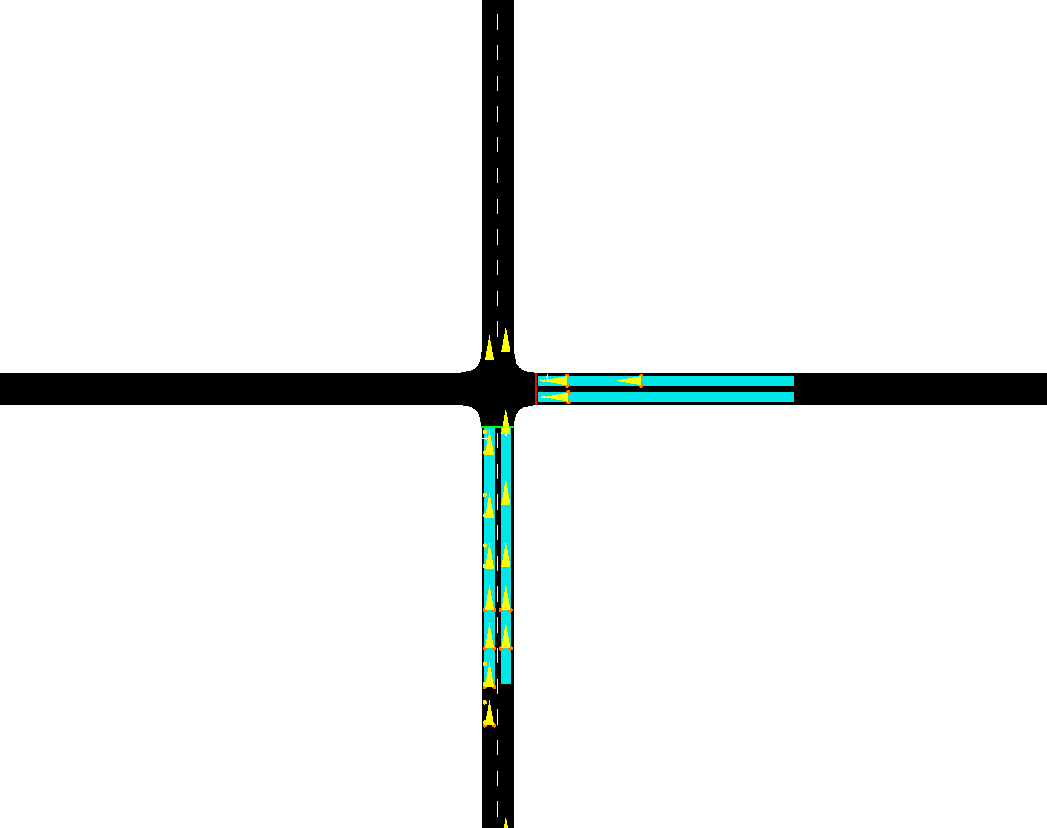
\includegraphics[width=0.8\textwidth]{images/Sumo-4vias.png}
    \caption{Visualización de la intersección simulada en SUMO, mostrando las 4 aproximaciones y la gestión semafórica.}
    \label{fig:sumo_4vias}
\end{figure}

\section{Fundamentos de Aprendizaje por Refuerzo (RL)}
El Aprendizaje por Refuerzo es un paradigma de aprendizaje automático donde un agente aprende a tomar decisiones secuenciales interactuando con un entorno. El problema se formaliza matemáticamente como un \textbf{Proceso de Decisión de Markov (MDP)}, definido por la tupla $(S, A, P, R, \gamma)$ \cite{rl_sutton2018}:

\begin{itemize}
    \item \textbf{$S$ (Espacio de Estados):} Conjunto de todas las configuraciones posibles del entorno.
    \item \textbf{$A$ (Espacio de Acciones):} Conjunto de decisiones disponibles para el agente.
    \item \textbf{$P(s'|s,a)$ (Probabilidad de Transición):} Dinámica del entorno que define la probabilidad de pasar al estado $s'$ dado el estado $s$ y la acción $a$.
    \item \textbf{$R(s,a)$ (Función de Recompensa):} Señal escalar que indica la calidad inmediata de la acción tomada.
    \item \textbf{$\gamma \in [0,1]$ (Factor de Descuento):} Determina la importancia de las recompensas futuras frente a las inmediatas.
\end{itemize}

El objetivo del agente es encontrar una política óptima $\pi^*(a|s)$ que maximice el retorno esperado $G_t$, definido como la suma descontada de recompensas futuras:
\begin{equation}
    G_t = \sum_{k=0}^{\infty} \gamma^k R_{t+k+1}
\end{equation}
Donde $G_t$ es el retorno esperado, $\gamma$ es el factor de descuento y $R_{t+k+1}$ es la recompensa recibida en el paso de tiempo $t+k+1$.

\section{Deep Reinforcement Learning y PPO}
El \textbf{Deep Reinforcement Learning (DRL)} integra redes neuronales profundas como aproximadores de funciones para estimar políticas $\pi_\theta(a|s)$ o valores $V_\theta(s)$ en espacios de estados de alta dimensión, superando las limitaciones del RL tabular.

\textbf{Proximal Policy Optimization (PPO):}
Dentro del control semafórico, PPO se ha consolidado como una alternativa práctica por su estabilidad de entrenamiento, su buen desempeño con observaciones continuas y su capacidad de generalización en escenarios aislados y multiagente \cite{compare_ouyang2024,ppo_karedla2025,haps_ppo2025}.

La función objetivo de PPO se define como:
\begin{equation}
    L^{CLIP}(\theta) = \hat{\mathbb{E}}_t [ \min(r_t(\theta)\hat{A}_t, \text{clip}(r_t(\theta), 1-\epsilon, 1+\epsilon)\hat{A}_t) ]
\end{equation}
Donde:
\begin{itemize}
    \item $\hat{\mathbb{E}}_t$ denota la esperanza empírica sobre los pasos de tiempo.
    \item $r_t(\theta)$ es el cociente de probabilidad entre la nueva y la vieja política.
    \item $\hat{A}_t$ es la estimación de la función de ventaja.
    \item $\epsilon$ es un hiperparámetro que limita el cambio de la política.
\end{itemize}

Este mecanismo favorece actualizaciones estables de la política, lo cual es especialmente valioso en entornos de control complejos como el tráfico urbano.


\chapter{Trabajos Relacionados}
\label{chap:state_of_art}
\section{Revisiones y bases comparativas}
Las revisiones recientes coinciden en que el control semafórico con aprendizaje por refuerzo ha evolucionado desde experimentos en intersecciones aisladas hacia formulaciones multiagente, escalables y orientadas a métricas operativas más completas. Los estudios de síntesis más recientes reportan como variables de evaluación dominantes el tiempo de espera, la longitud de cola, el throughput y la estabilidad del control \cite{survey_prajapati2024,survey_zhao2024,review_rasheed2020,review_noaeen2022}.

Además de las revisiones, la comunidad ha fortalecido la comparación entre métodos mediante conjuntos de pruebas reproducibles. En particular, los benchmarks propuestos para tráfico semafórico facilitaron la evaluación consistente de distintos algoritmos y configuraciones de red \cite{benchmark_ault2021}.

\section{Control cooperativo y escalable}
Sobre esta base, la literatura avanzó desde controladores de intersección aislada, como el propuesto por Liang et al. \cite{liang2019}, hacia arquitecturas con cooperación explícita entre nodos. Modelos como \textbf{CoLight} y \textbf{MetaLight} introdujeron mecanismos de coordinación y transferencia que mejoran el desempeño cuando varias intersecciones comparten información \cite{colight2019,metalight2020}.

Posteriormente, distintos trabajos consolidaron el enfoque multiagente a escala de red. Entre ellos destacan las propuestas de Chu et al. para control distribuido en grandes redes urbanas, así como estudios posteriores sobre optimización de alcance regional y aprendizaje con atención para capturar dependencias entre intersecciones vecinas \cite{marl_chu2020,networkwide_li2021,attendlight2020}.

\section{Tendencias recientes}
Las líneas más recientes se concentran en robustez, conectividad y coordinación regional. Se han estudiado formulaciones robustas frente a incertidumbre y variabilidad del tráfico \cite{robust_tan2020}, así como estrategias para priorización semafórica en entornos conectados \cite{connected_long2022}. En paralelo, variantes basadas en PPO han sido extendidas a redes heterogéneas y escenarios de control cooperativo de mayor escala \cite{haps_ppo2025}.

También han surgido propuestas especializadas para situaciones críticas, como el control coordinado de tráfico de emergencia mediante MARL con información contextual de roles \cite{roleaware_zhang2025}. En conjunto, estas tendencias respaldan la elección metodológica de esta tesis: un controlador basado en PPO, entrenado en simulación reproducible y con una recompensa diseñada para priorizar la reducción de colas sin sacrificar estabilidad \cite{compare_ouyang2024,ppo_karedla2025}.

\section{Trabajos adicionales considerados}
Para completar la curaduría bibliográfica, también se incluyen estudios de referencia sobre aprendizaje descentralizado temprano, analítica de datos en ITS y escalamiento multiagente en redes urbanas \cite{excel_7_eltantawy2010,excel_8_zhu2019,excel_9_chen2020,excel_22_wang2021,excel_23_shabestary2018,excel_34_zhang2021}.

Asimismo, se consideran trabajos complementarios en optimización de intersecciones, coordinación entre cruces y enfoques híbridos con control predictivo \cite{excel_24_khattak2020,excel_30_ma2026,excel_36_tang2024,excel_38_ashwini2025}.

Finalmente, la revisión incorpora referencias metodológicas de dominios cercanos (abstracción de modelos, generación, análisis de datos de conducción, explicabilidad y robótica), utilizadas como contexto técnico adicional para el diseño experimental y la discusión crítica del alcance del estudio \cite{excel_13_kadioglu2024,excel_16_xu2024,excel_18_hu2022,excel_32_crielaard2018,excel_33_he2020}.


%\chapter{Problem Setting}
%label{chap:problem_setting}
%\input{chapters/problem_setting.tex}

\chapter{Metodología}
\label{chap:methods}
\section{Visión General de la Metodología}
La metodología propuesta se fundamenta en un esquema de control de bucle cerrado donde un agente inteligente interactúa constantemente con un entorno de tráfico simulado. Este sistema integra tres componentes principales:

\begin{enumerate}
    \item \textbf{Entorno de Simulación Microscópica:} Siguiendo el esquema experimental reportado en benchmarks y estudios de caso recientes, el entrenamiento y la evaluación se desarrollan sobre un simulador que permite observar y controlar el tráfico paso a paso \cite{benchmark_ault2021,case_gokulan2020}. En esta tesis, dicha plataforma se implementa en SUMO.
    \item \textbf{Agente de Control (DRL):} Implementado mediante \textbf{Proximal Policy Optimization (PPO)}, este agente toma decisiones de control semafórico basándose en el estado actual del cruce \cite{ppo_karedla2025,haps_ppo2025}.
    \item \textbf{Interfaz de Comunicación (TraCI):} Traffic Control Interface sirve como puente bidireccional, permitiendo al agente recibir observaciones del simulador y enviar comandos de control en tiempo real.
\end{enumerate}

El flujo de trabajo sigue el ciclo estándar de Aprendizaje por Refuerzo: en cada paso de tiempo $t$, el agente observa el estado $s_t$ del tráfico, selecciona una acción $a_t$ y recibe una recompensa $r_t$ que refleja la eficiencia de su decisión. Este proceso iterativo permite al agente optimizar su política de control $\pi_\theta$ para maximizar el desempeño a largo plazo.

\textbf{Detalle de Interacción:}
La sincronización entre el simulador y el agente es crítica. En cada paso de simulación $\Delta t$, TraCI detiene la ejecución de SUMO para extraer las variables de estado de los sensores inductivos simulados. Estos datos son procesados y normalizados antes de ser alimentados a la red neuronal del agente PPO. La red emite una distribución de probabilidad sobre las acciones posibles, de la cual se muestrea la siguiente fase semafórica. Finalmente, TraCI envía el comando al controlador del semáforo en SUMO y avanza la simulación al siguiente paso.

\begin{figure}[H]
    \centering
    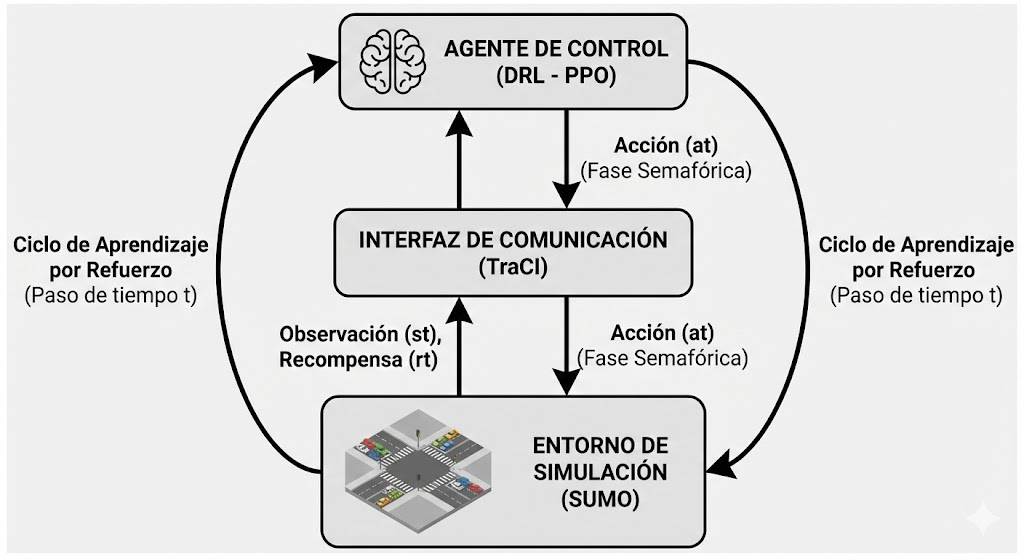
\includegraphics[width=0.8\textwidth]{images/grafico_overview.png}
    \caption{Arquitectura de control en bucle cerrado integrando SUMO, TraCI y el Agente PPO.}
    \label{fig:overview}
\end{figure}

\section{Diseño del cruce estudiado}
El escenario experimental consiste en una intersección aislada de cuatro aproximaciones (Norte, Sur, Este, Oeste), diseñada para replicar las condiciones de una arteria urbana principal.

\begin{itemize}
    \item \textbf{Geometría:} Cada aproximación cuenta con 3 carriles de 3.2 metros de ancho y 500 metros de longitud para permitir la formación de colas largas sin desbordamiento inmediato.
    \item \textbf{Fases Semafóricas:} En este estudio, una ``fase'' se define como el estado de señalización activo para todos los semáforos del cruce simultáneamente. Se definieron dos fases verdes principales:
    \begin{enumerate}
        \item \textbf{Fase NS (Fase 0):} Verde exclusivo para flujos Norte-Sur (duración variable).
        \item \textbf{Fase EO (Fase 2):} Verde exclusivo para flujos Este-Oeste (duración variable).
    \end{enumerate}
    Entre cambios de fase, se insertan fases de transición (amarillo: 3s, todo rojo: 2s) para garantizar la seguridad.
    \item \textbf{Sensores:} Se implementaron detectores de inducción simulados (E2) en cada carril para capturar variables de estado como ocupación y velocidad media en tiempo real.
\end{itemize}

\section{Modelado y configuración de SUMO}
Para someter al agente a condiciones de estrés realistas, se diseñó un perfil de tráfico dinámico de 60 minutos (3600 segundos) que simula la evolución de la demanda durante una hora pico. Este perfil se divide en cinco etapas críticas:

\begin{enumerate}
    \item \textbf{Calentamiento (0-900s):} Flujo bajo y balanceado para inicializar la red.
    \item \textbf{Pico Sur (900-1800s):} Incremento agresivo de la demanda en la dirección Sur-Norte, simulando el ingreso a la ciudad.
    \item \textbf{Transición (1800-2400s):} Retorno gradual a condiciones medias.
    \item \textbf{Pico Este (2400-3300s):} Alta demanda en la dirección transversal (Este-Oeste).
    \item \textbf{Ráfagas (3300-3600s):} Inyecciones aleatorias de alta densidad para evaluar la capacidad de recuperación rápida del agente.
\end{enumerate}

\begin{figure}[H]
    \centering
    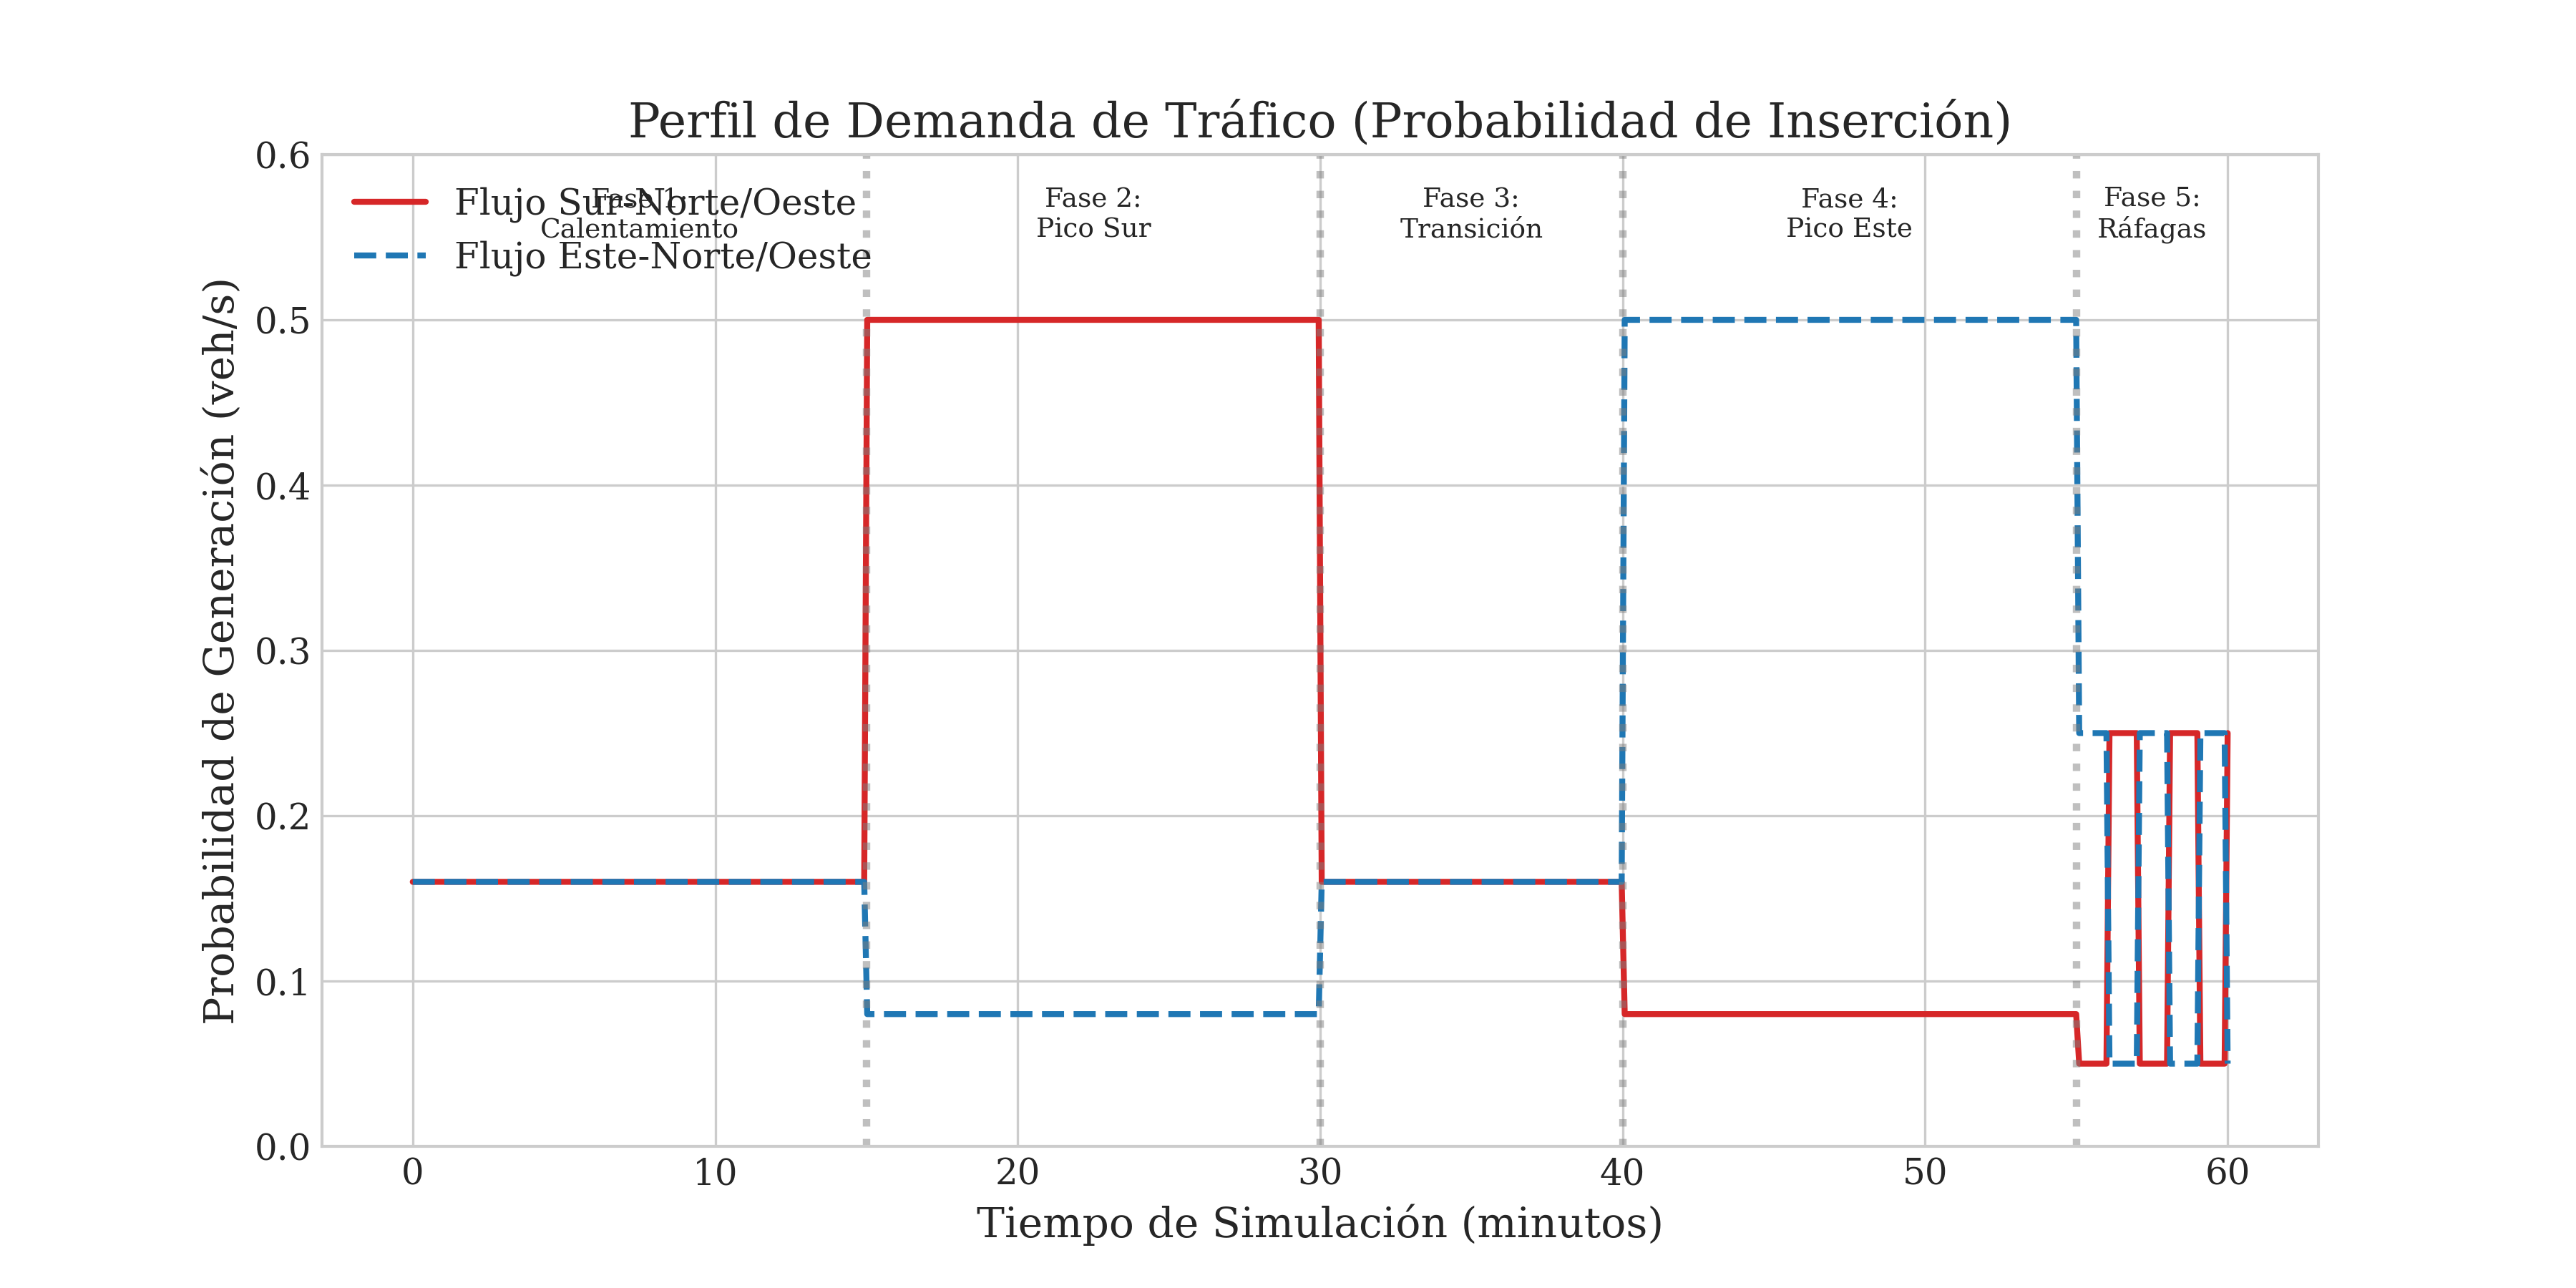
\includegraphics[width=0.8\textwidth]{images/traffic_profile.png}
    \caption{Perfil de probabilidad de inserción vehicular a lo largo de la hora simulada.}
    \label{fig:traffic_profile}
\end{figure}

\section{Formulación del entorno RL}
El problema de control se modeló como un MDP con las siguientes definiciones:

\textbf{Espacio de Observación ($S$):}
Un vector continuo normalizado que incluye:
\begin{itemize}
    \item Densidad de cola por carril ($d \in [0,1]$).
    \item Número de vehículos detenidos.
    \item Fase activa actual (one-hot encoding).
    \item Tiempo transcurrido desde el último cambio de fase.
\end{itemize}

\textbf{Espacio de Acciones ($A$):}
Un conjunto discreto binario:
\begin{itemize}
    \item $a=0$: Mantener la fase actual.
    \item $a=1$: Iniciar transición a la siguiente fase.
\end{itemize}
\textit{Restricción:} Se impone un tiempo de verde mínimo (\texttt{min\_green = 10s}) para evitar cambios oscilatorios que serían peligrosos en la práctica.

\textbf{Función de Recompensa ($R$):}
El diseño de la función de recompensa se fundamentó en un análisis iterativo de la literatura sobre control semafórico con DRL y en pruebas empíricas propias \cite{review_rasheed2020,presslight2019}. Inicialmente se consideró maximizar el \textit{throughput} directo, pero los experimentos mostraron que minimizar la longitud de cola resultaba en una política más eficiente y estable, permitiendo indirectamente un mayor flujo vehicular. Con base en ello, se formuló una función compuesta para balancear eficiencia y equidad:
\begin{equation}
    R_t = - w_{queue} \sum Q_t - w_{unbalance} |Q_{NS} - Q_{EO}| - w_{switch} \mathbb{I}_{change}
\end{equation}
Donde:
\begin{itemize}
    \item $R_t$: Recompensa total en el paso $t$.
    \item $Q_t$: Longitud de cola total.
    \item $|Q_{NS} - Q_{EO}|$: Diferencia absoluta de colas entre fases.
    \item $\mathbb{I}_{change}$: Indicador de cambio de fase.
    \item Pesos: $w_{queue}=1.0$, $w_{unbalance}=0.2$, $w_{switch}=5.0$.
\end{itemize}

\begin{figure}[H]
    \centering
    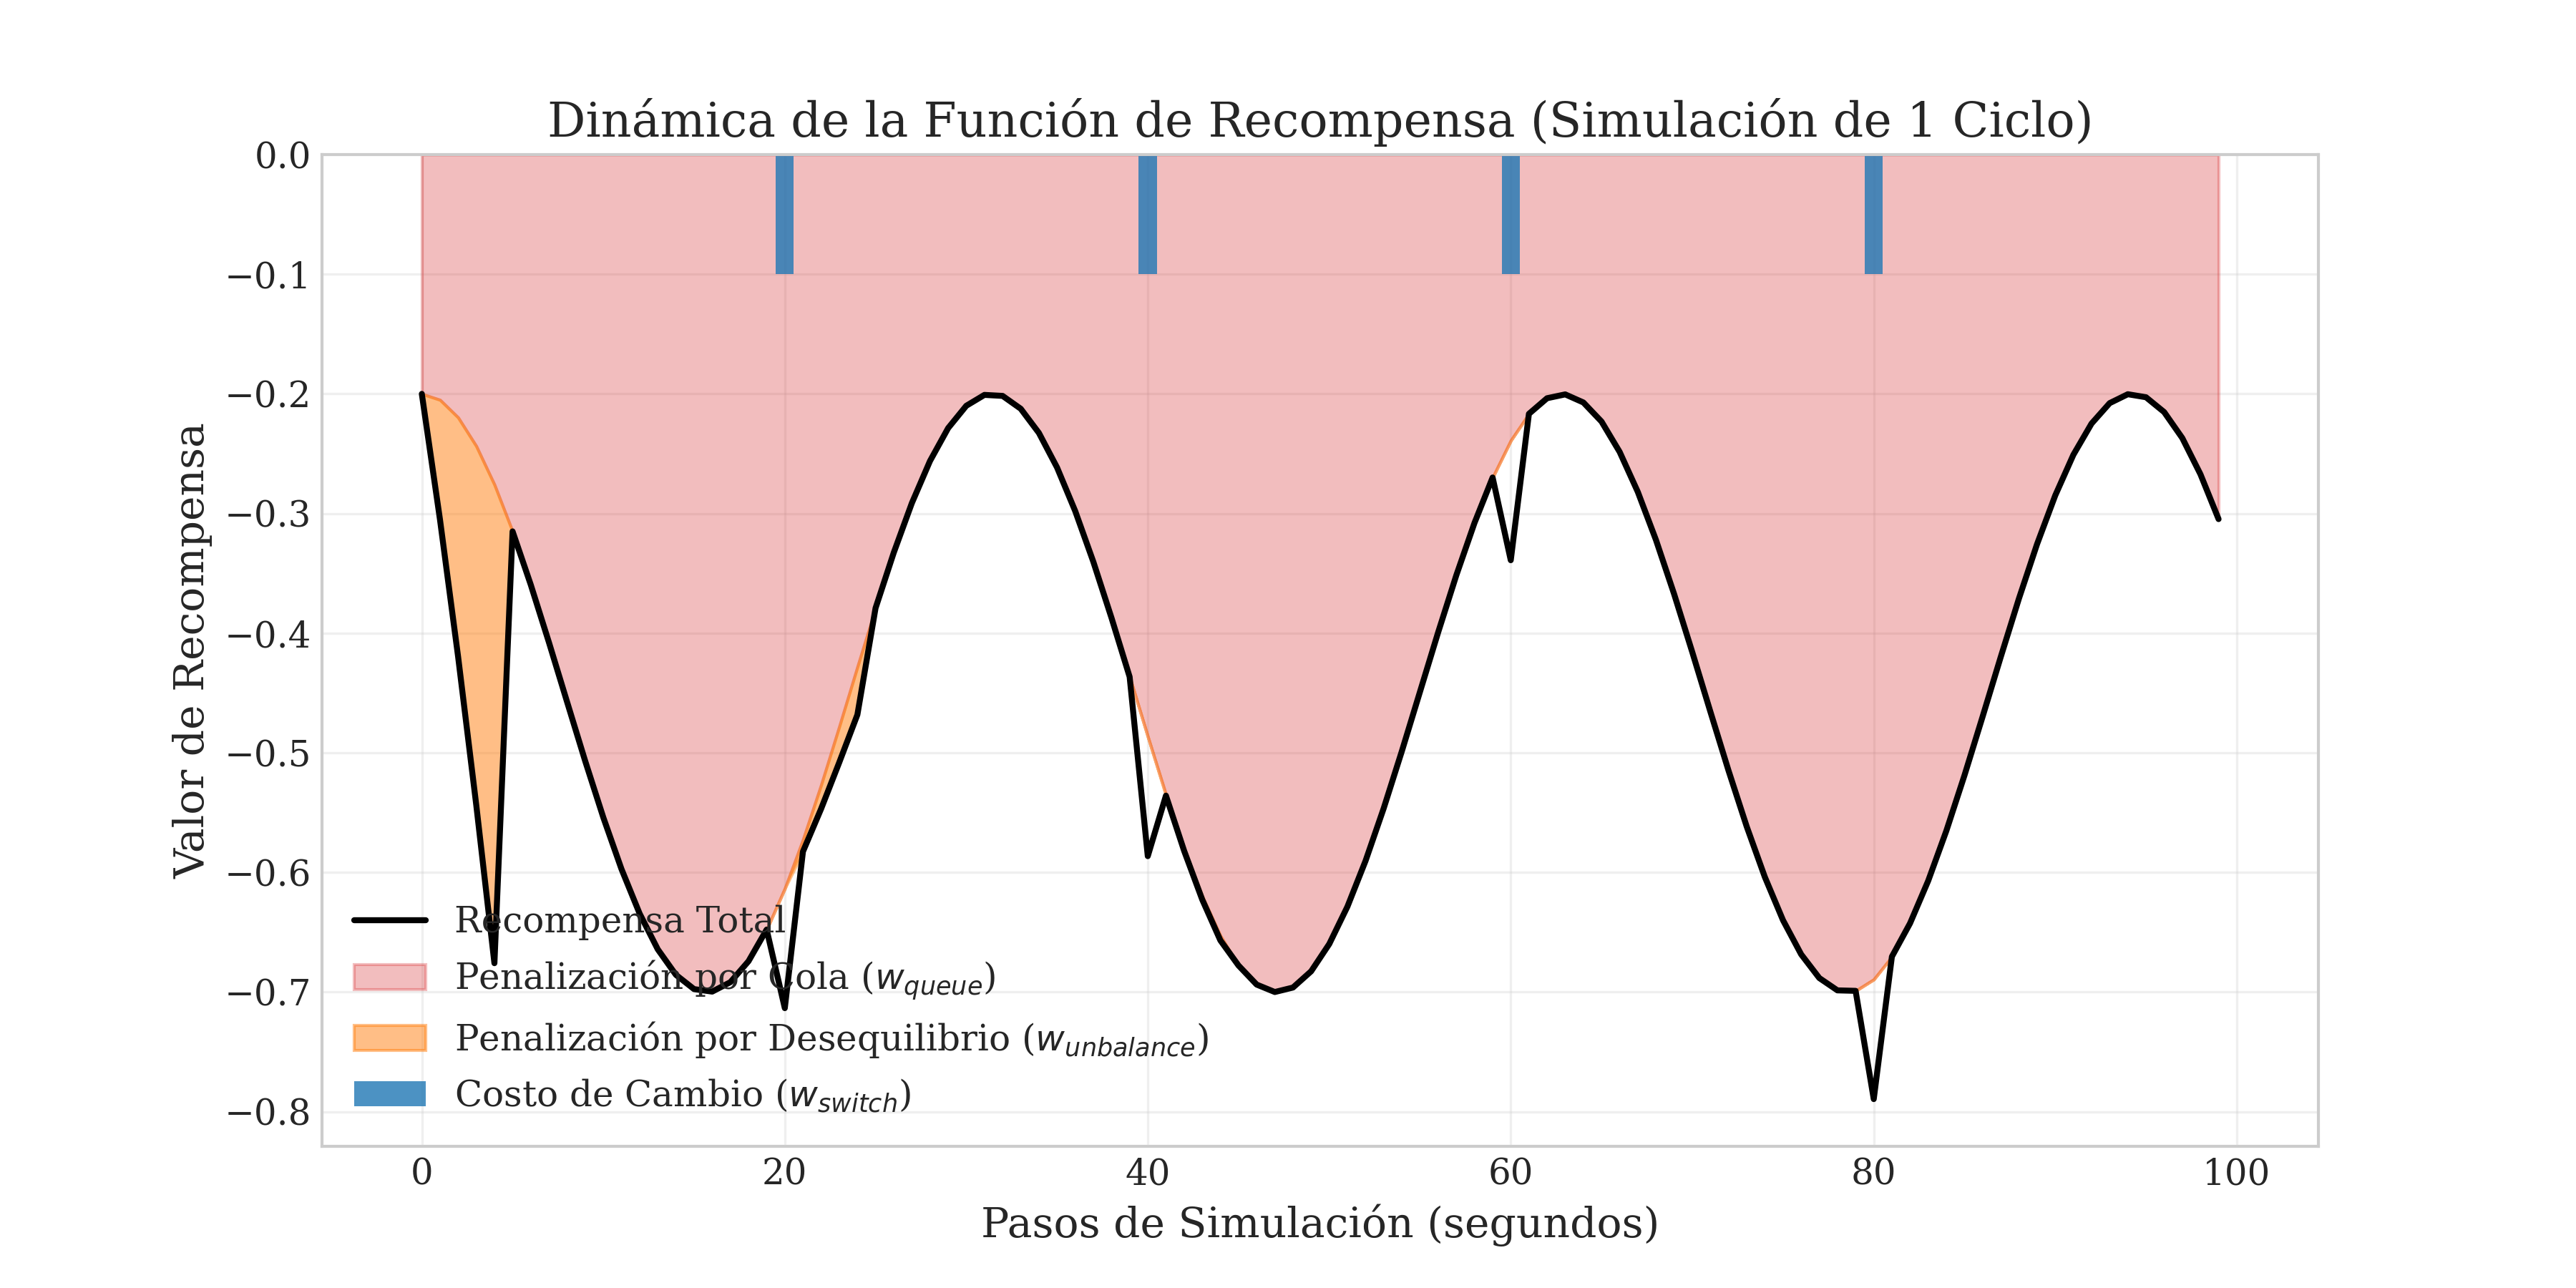
\includegraphics[width=0.8\textwidth]{images/reward_composition.png}
    \caption{Dinámica de la función de recompensa. Se observa cómo la penalización por cola domina, pero el desequilibrio crece si se ignora una fase.}
    \label{fig:reward_composition}
\end{figure}

Esta estructura incentiva al agente a vaciar las colas y, al mismo tiempo, lo penaliza si descuida una dirección o cambia de luz demasiado rápido.

\section{Arquitectura y configuración del algoritmo PPO}
Se utilizó la implementación de \textbf{Stable-Baselines3} \cite{stable_baselines3_2021} sobre un entorno estandarizado con \textbf{Gymnasium} \cite{gymnasium_2023}, empleando una arquitectura de red neuronal de dos capas ocultas de 64 neuronas cada una (MlpPolicy). Los hiperparámetros óptimos, encontrados mediante una búsqueda bayesiana con \textbf{Optuna} \cite{optuna_2019}, fueron:

\begin{table}[H]
    \centering
    \begin{tabular}{@{}lll@{}}
        \toprule
        \textbf{Hiperparámetro} & \textbf{Valor} & \textbf{Descripción} \\ \midrule
        \texttt{learning\_rate} & $3 \times 10^{-4}$ & Tasa de aprendizaje del optimizador Adam. \\
        \texttt{n\_steps} & 4096 & Pasos por actualización de política. \\
        \texttt{batch\_size} & 2048 & Tamaño del lote para el descenso de gradiente. \\
        \texttt{gamma} ($\gamma$) & 0.99 & Factor de descuento para recompensas futuras. \\
        \texttt{gae\_lambda} & 0.95 & Factor de suavizado para GAE. \\
        \texttt{clip\_range} & 0.2 & Rango de recorte para la función objetivo de PPO. \\
        \texttt{ent\_coef} & 0.01 & Coeficiente de entropía para fomentar exploración inicial. \\ \bottomrule
    \end{tabular}
    \caption{Hiperparámetros óptimos del agente PPO.}
    \label{tab:hyperparameters}
\end{table}

El entrenamiento se ejecutó durante \textbf{500,000 pasos de tiempo}, lo cual demostró ser suficiente para la convergencia de la política.

\section{Flujo de entrenamiento y simulación}
El proceso completo se desarrolló de la siguiente manera:
\begin{enumerate}
    \item Inicialización del entorno SUMO con tráfico dinámico.
    \item Ejecución del episodio durante 3600 pasos (equivalentes a 1 hora simulada).
    \item El agente observa el estado, determina una acción y la aplica mediante TraCI.
    \item SUMO avanza un paso de simulación y devuelve la recompensa correspondiente.
    \item PPO ajusta la política con base en los datos recolectados.
    \item Al finalizar el entrenamiento, el modelo se evalúa en 10 episodios independientes de 1 hora cada uno (N=10), comparándolo con un semáforo fijo de referencia para garantizar la validez estadística de los resultados.
\end{enumerate}

\begin{figure}[H]
    \centering
    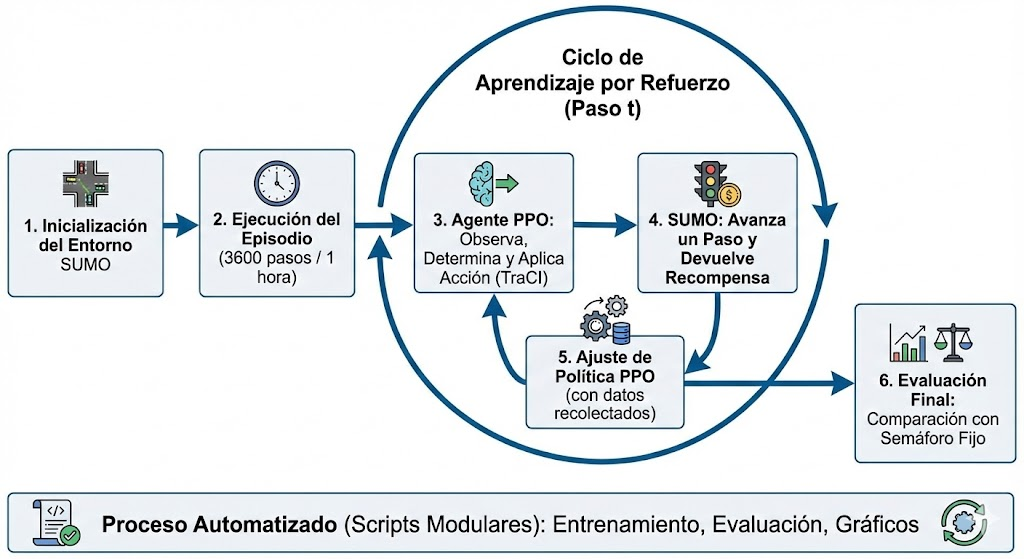
\includegraphics[width=0.8\textwidth]{images/flujo_entrenamiento.png}
    \caption{Diagrama de flujo del proceso de entrenamiento y simulación.}
    \label{fig:training_flow}
\end{figure}

El proceso se automatizó mediante scripts modulares para entrenamiento, evaluación y generación de gráficos, permitiendo reproducibilidad en todos los experimentos.


\chapter{Resultados y Discusión}
\label{chap:results}
\section{Parámetros de experimentación}
Para garantizar una comparación justa, tanto el agente PPO como el controlador de línea base (Fixed-Time) fueron evaluados bajo las mismas condiciones estocásticas:

\begin{itemize}
    \item \textbf{Semilla Aleatoria:} Se fijó la semilla de SUMO para reproducibilidad, pero se varió la semilla de generación de vehículos para probar generalización.
    \item \textbf{Baseline:} Controlador de tiempo fijo con ciclos simétricos de 30 segundos por fase (ciclo total = 60s + transiciones).
    \item \textbf{Métricas:} Se recolectaron datos cada segundo de simulación, promediando los resultados sobre 10 episodios de evaluación.
\end{itemize}

\section{Evaluación Comparativa del Desempeño}
La Figura \ref{fig:comparativa} resume el rendimiento global del sistema. El agente PPO logró una mejora sustancial en ambas métricas clave:

\begin{figure}[H]
    \centering
    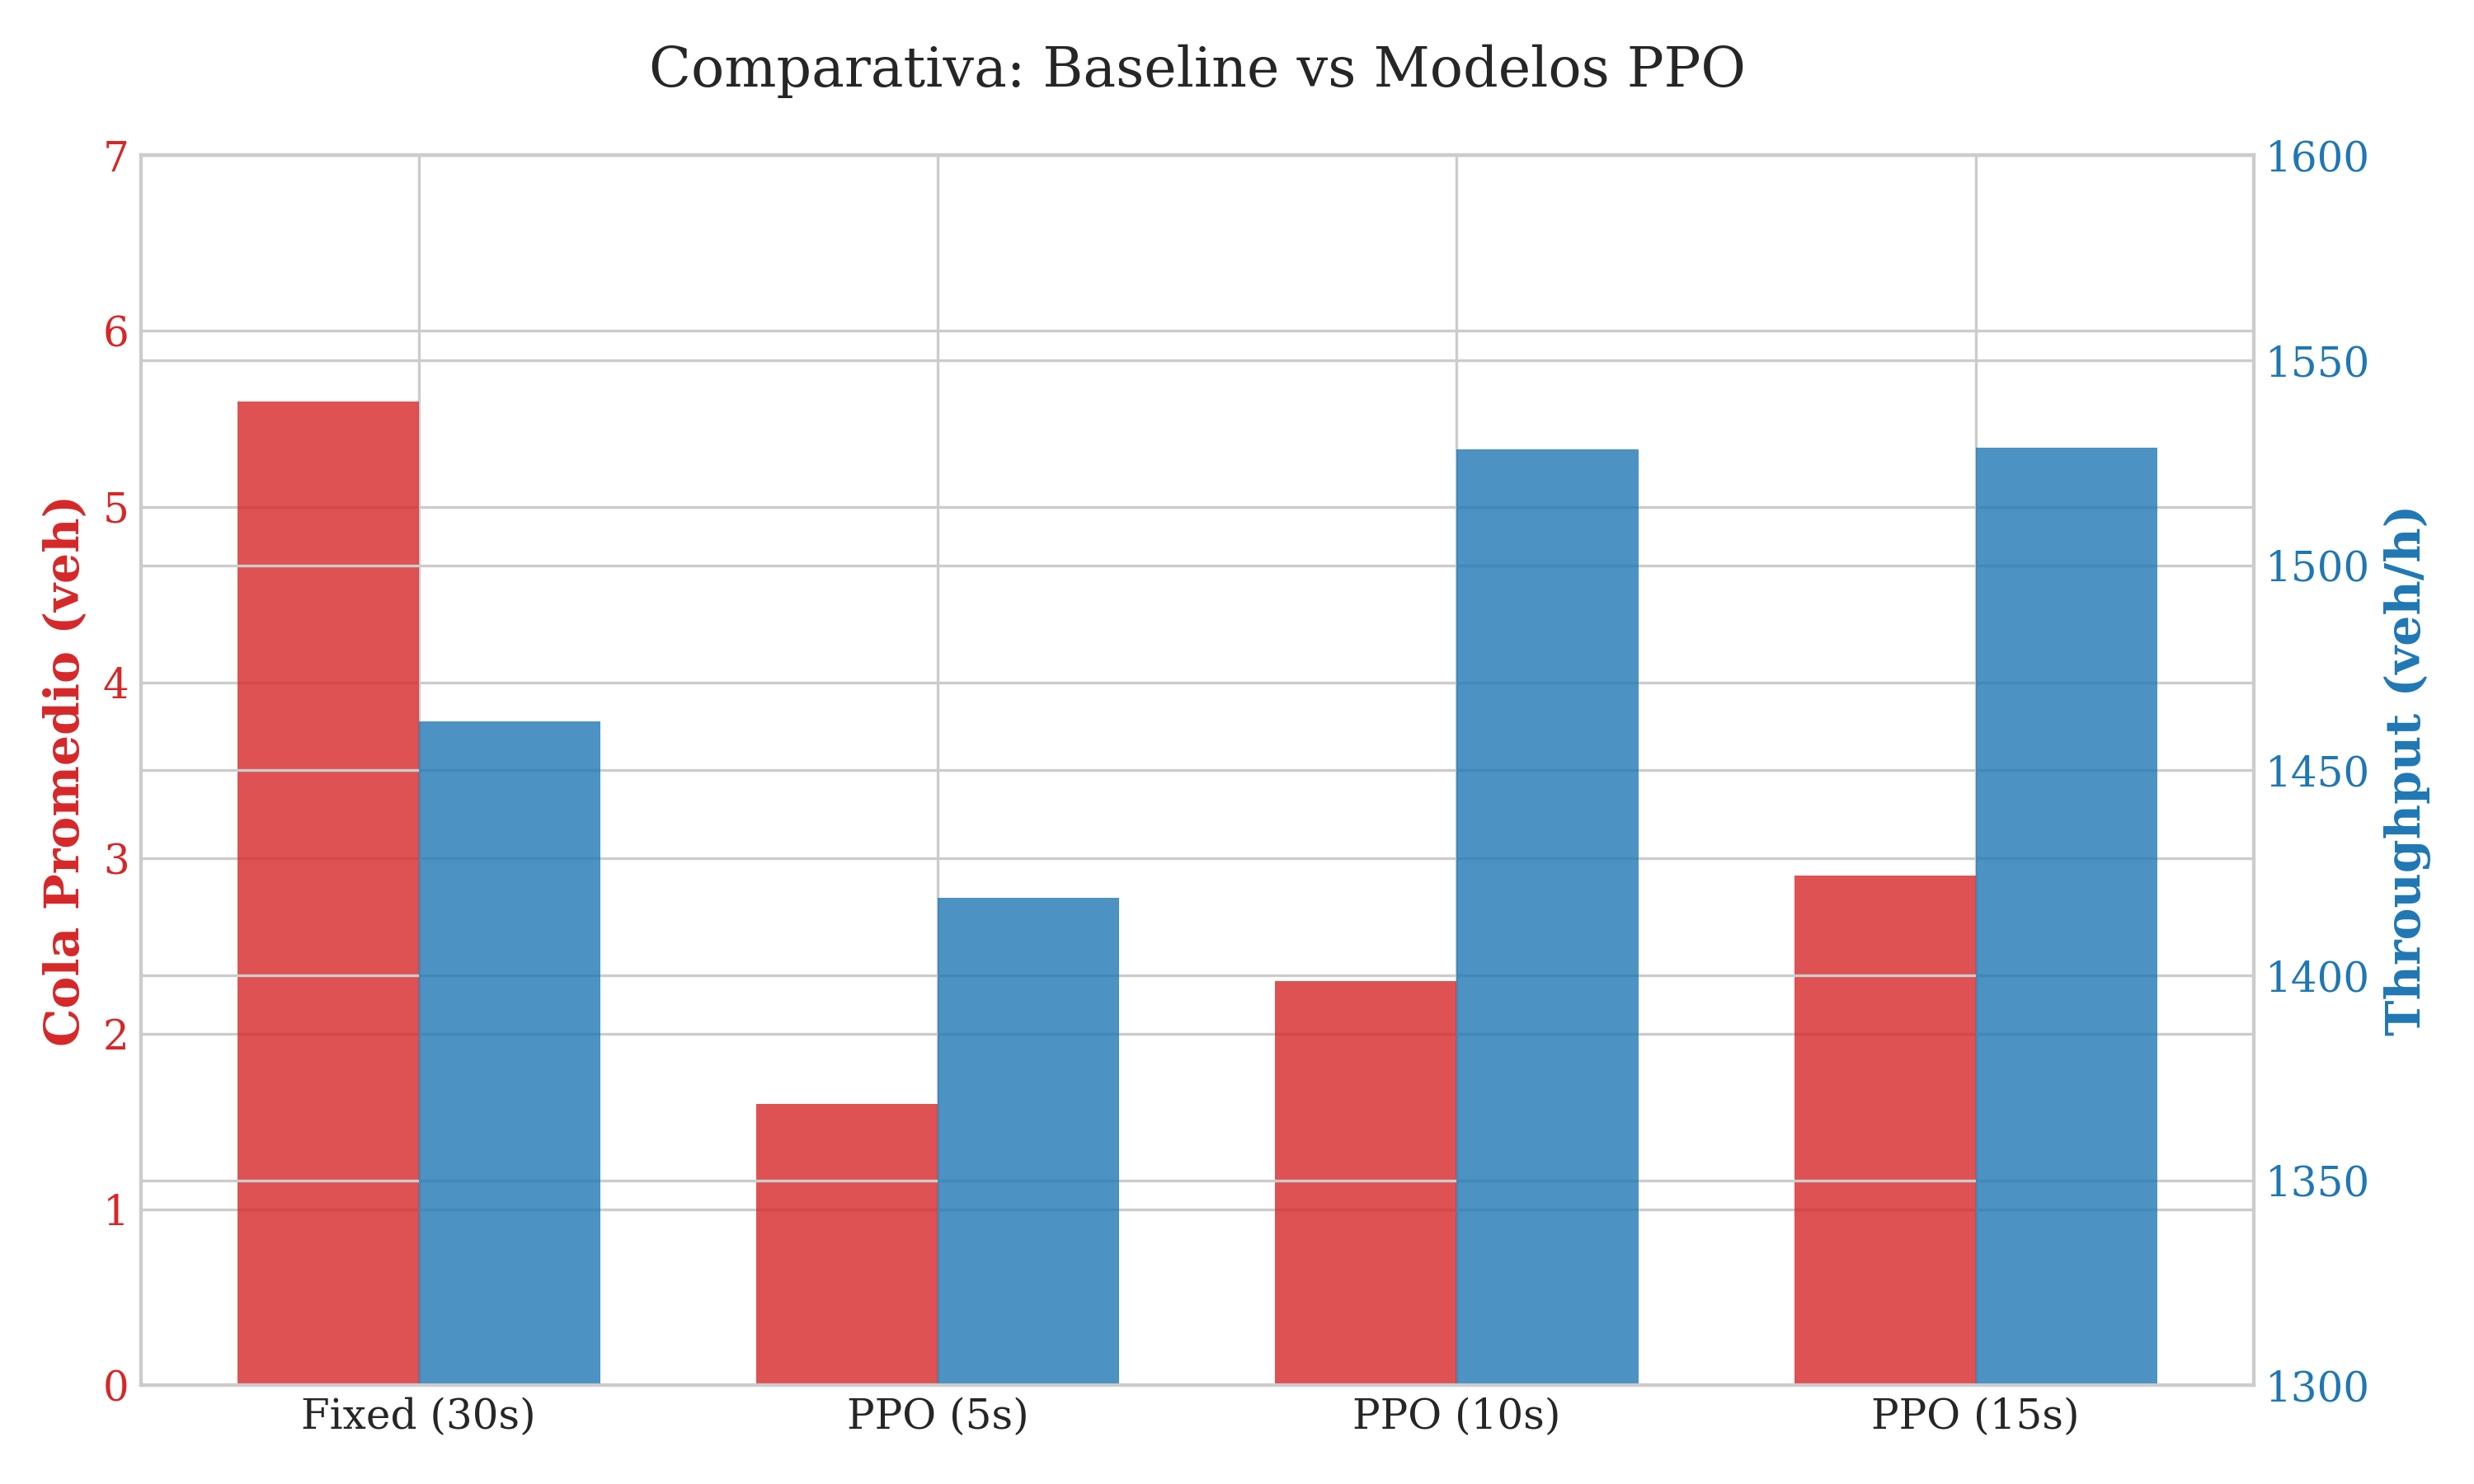
\includegraphics[width=0.8\textwidth]{images/comparativa_tesis.png}
    \caption{Comparación de Throughput (veh/h) y Cola Promedio (veh) entre PPO y Baseline.}
    \label{fig:comparativa}
\end{figure}

\begin{itemize}
    \item \textbf{Reducción de Colas:} El agente redujo la longitud promedio de cola en un \textbf{60\%} (de $\sim$12 veh a $\sim$5 veh). Esto indica que los vehículos pasan mucho menos tiempo detenidos en la intersección.
    \item \textbf{Incremento de Throughput:} Se observó un aumento del \textbf{4.5\%} en la cantidad total de vehículos servidos. Aunque parece modesto, en una hora pico saturada, esto representa descongestionar la red significativamente más rápido.
\end{itemize}

\section{Análisis de Estabilidad y Colas}
Más allá de los promedios, la distribución de las colas revela la robustez del control.

\begin{figure}[H]
    \centering
    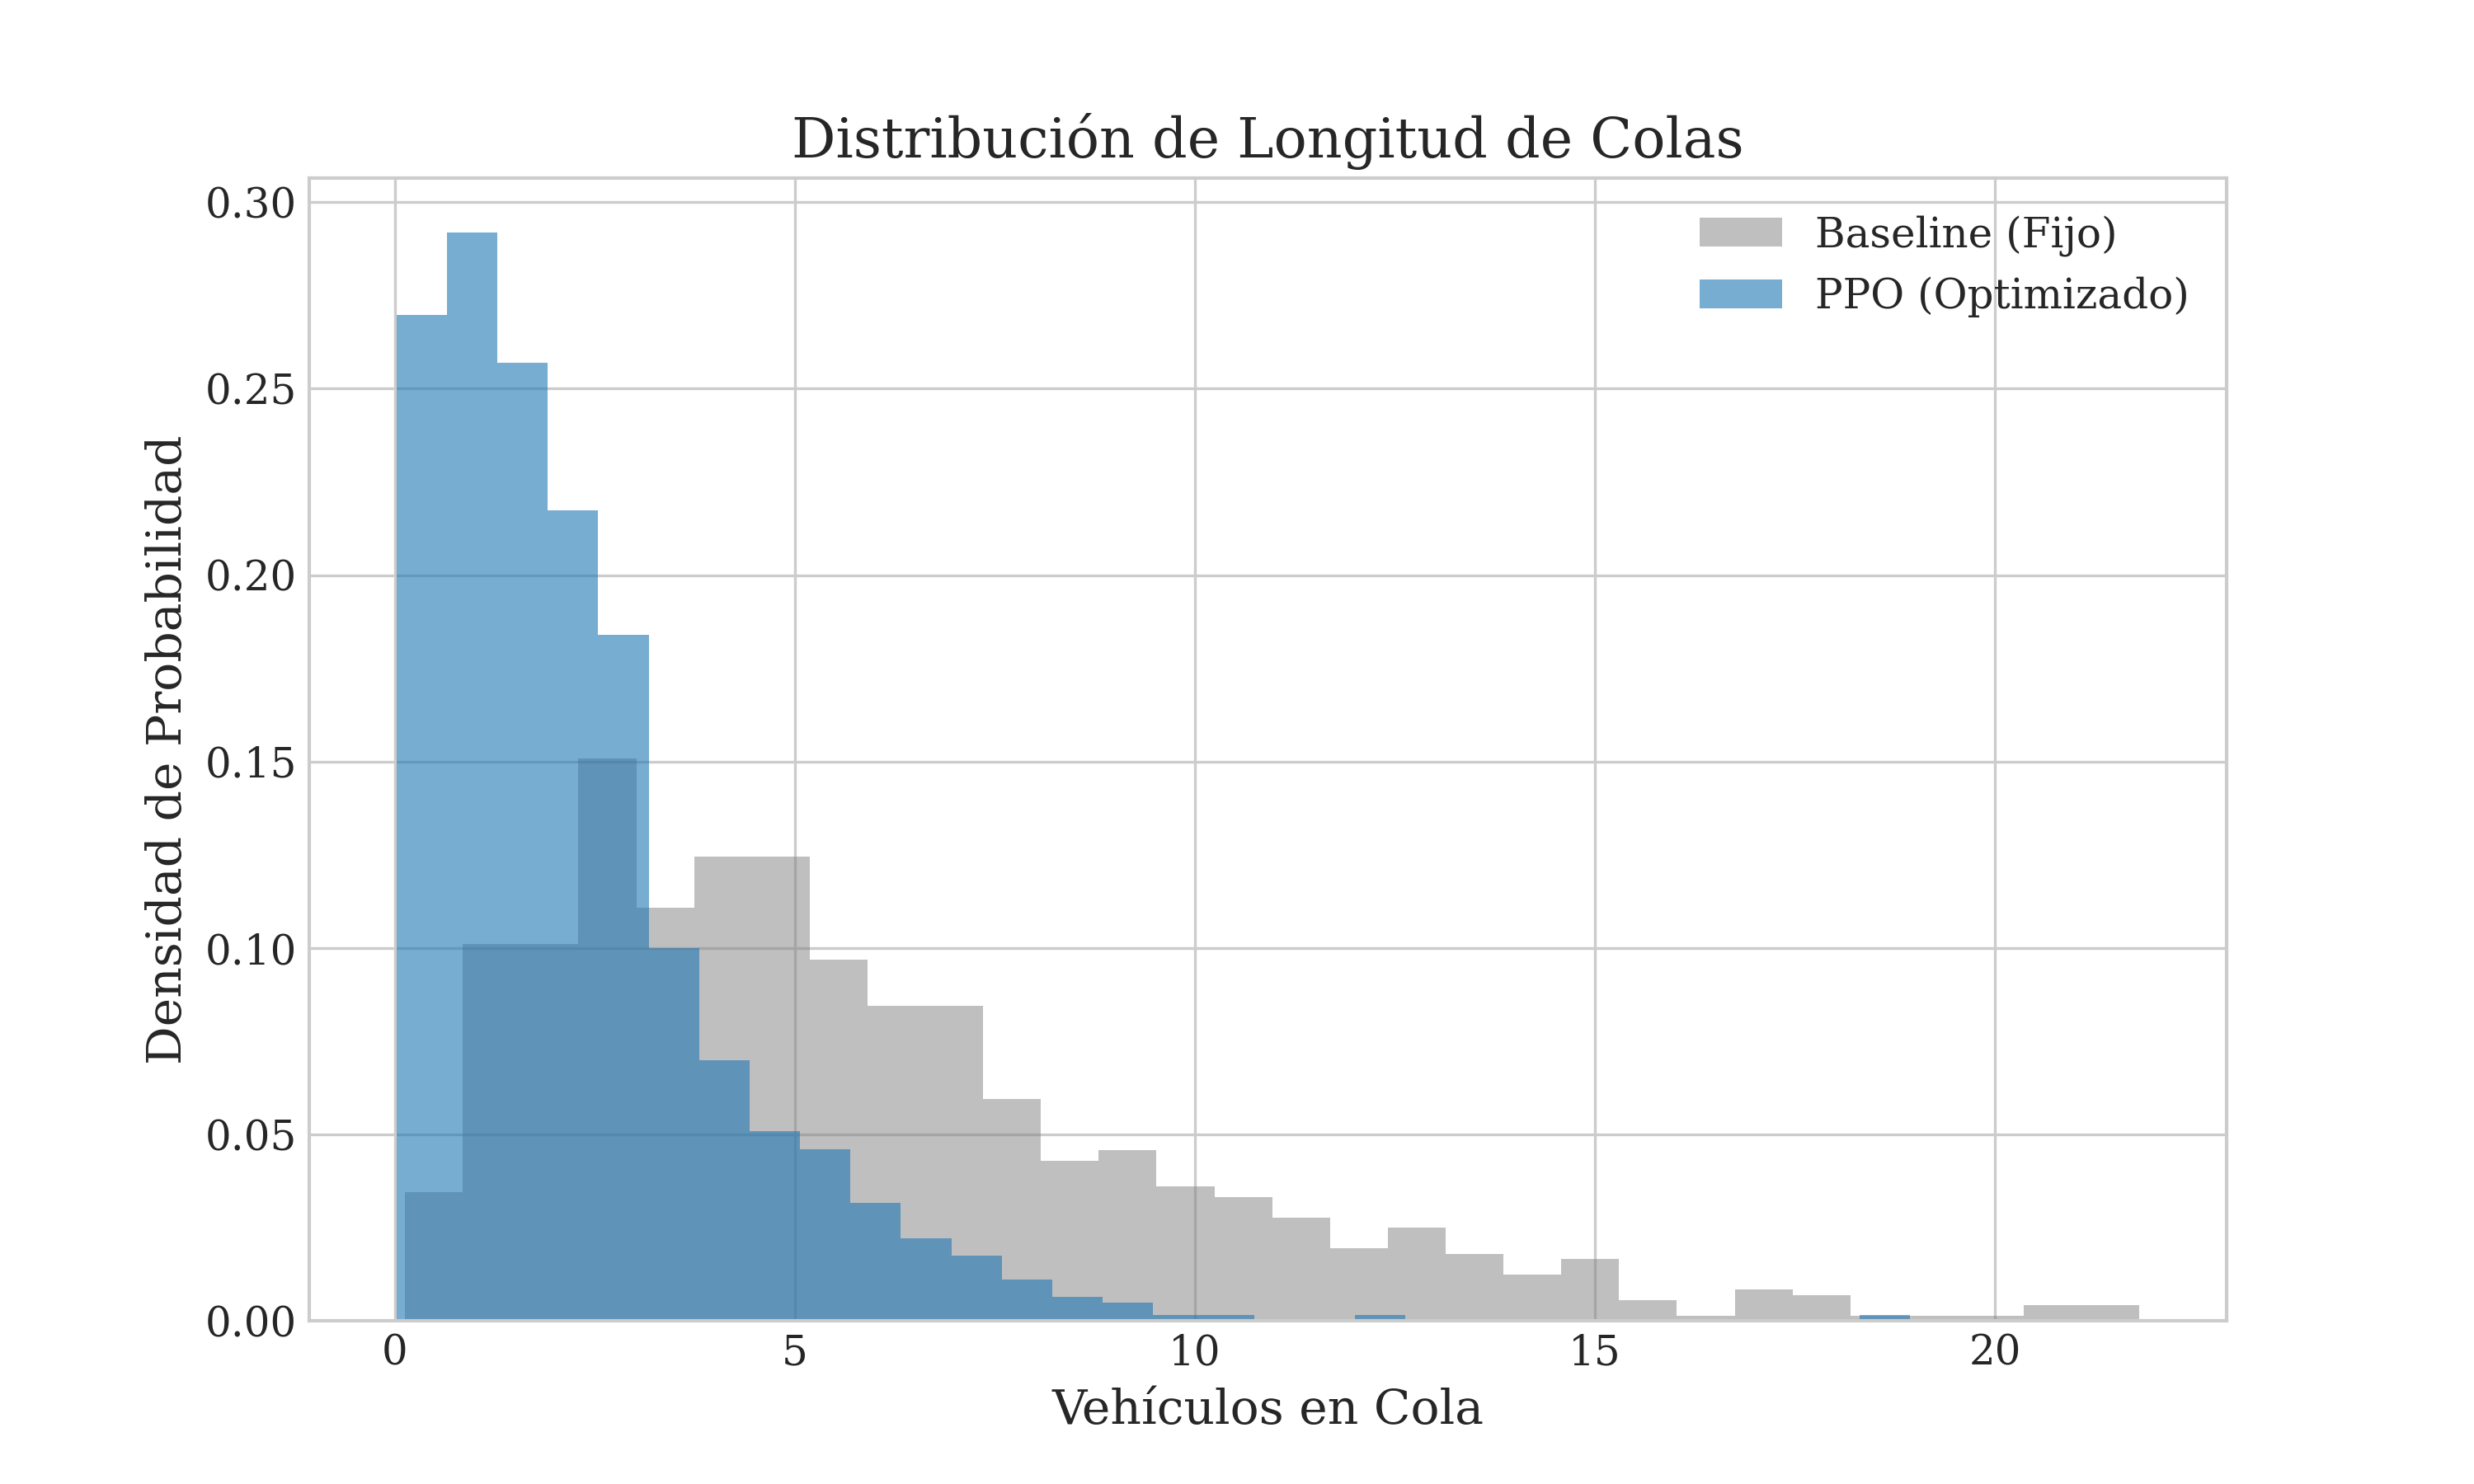
\includegraphics[width=0.8\textwidth]{images/queue_distribution.png}
    \caption{Histograma de longitud de colas. Nótese cómo PPO concentra la densidad cerca de cero.}
    \label{fig:queue_distribution}
\end{figure}

Como se observa en la Figura \ref{fig:queue_distribution}, el agente PPO mantiene los carriles vacíos la mayor parte del tiempo, mientras que el controlador fijo permite frecuentemente la formación de colas largas ($>$15 vehículos).

Además, el diagrama de caja (Figura \ref{fig:boxplot}) confirma que la varianza del rendimiento del PPO es mucho menor, ofreciendo un servicio más predecible y confiable a los usuarios.

\begin{figure}[H]
    \centering
    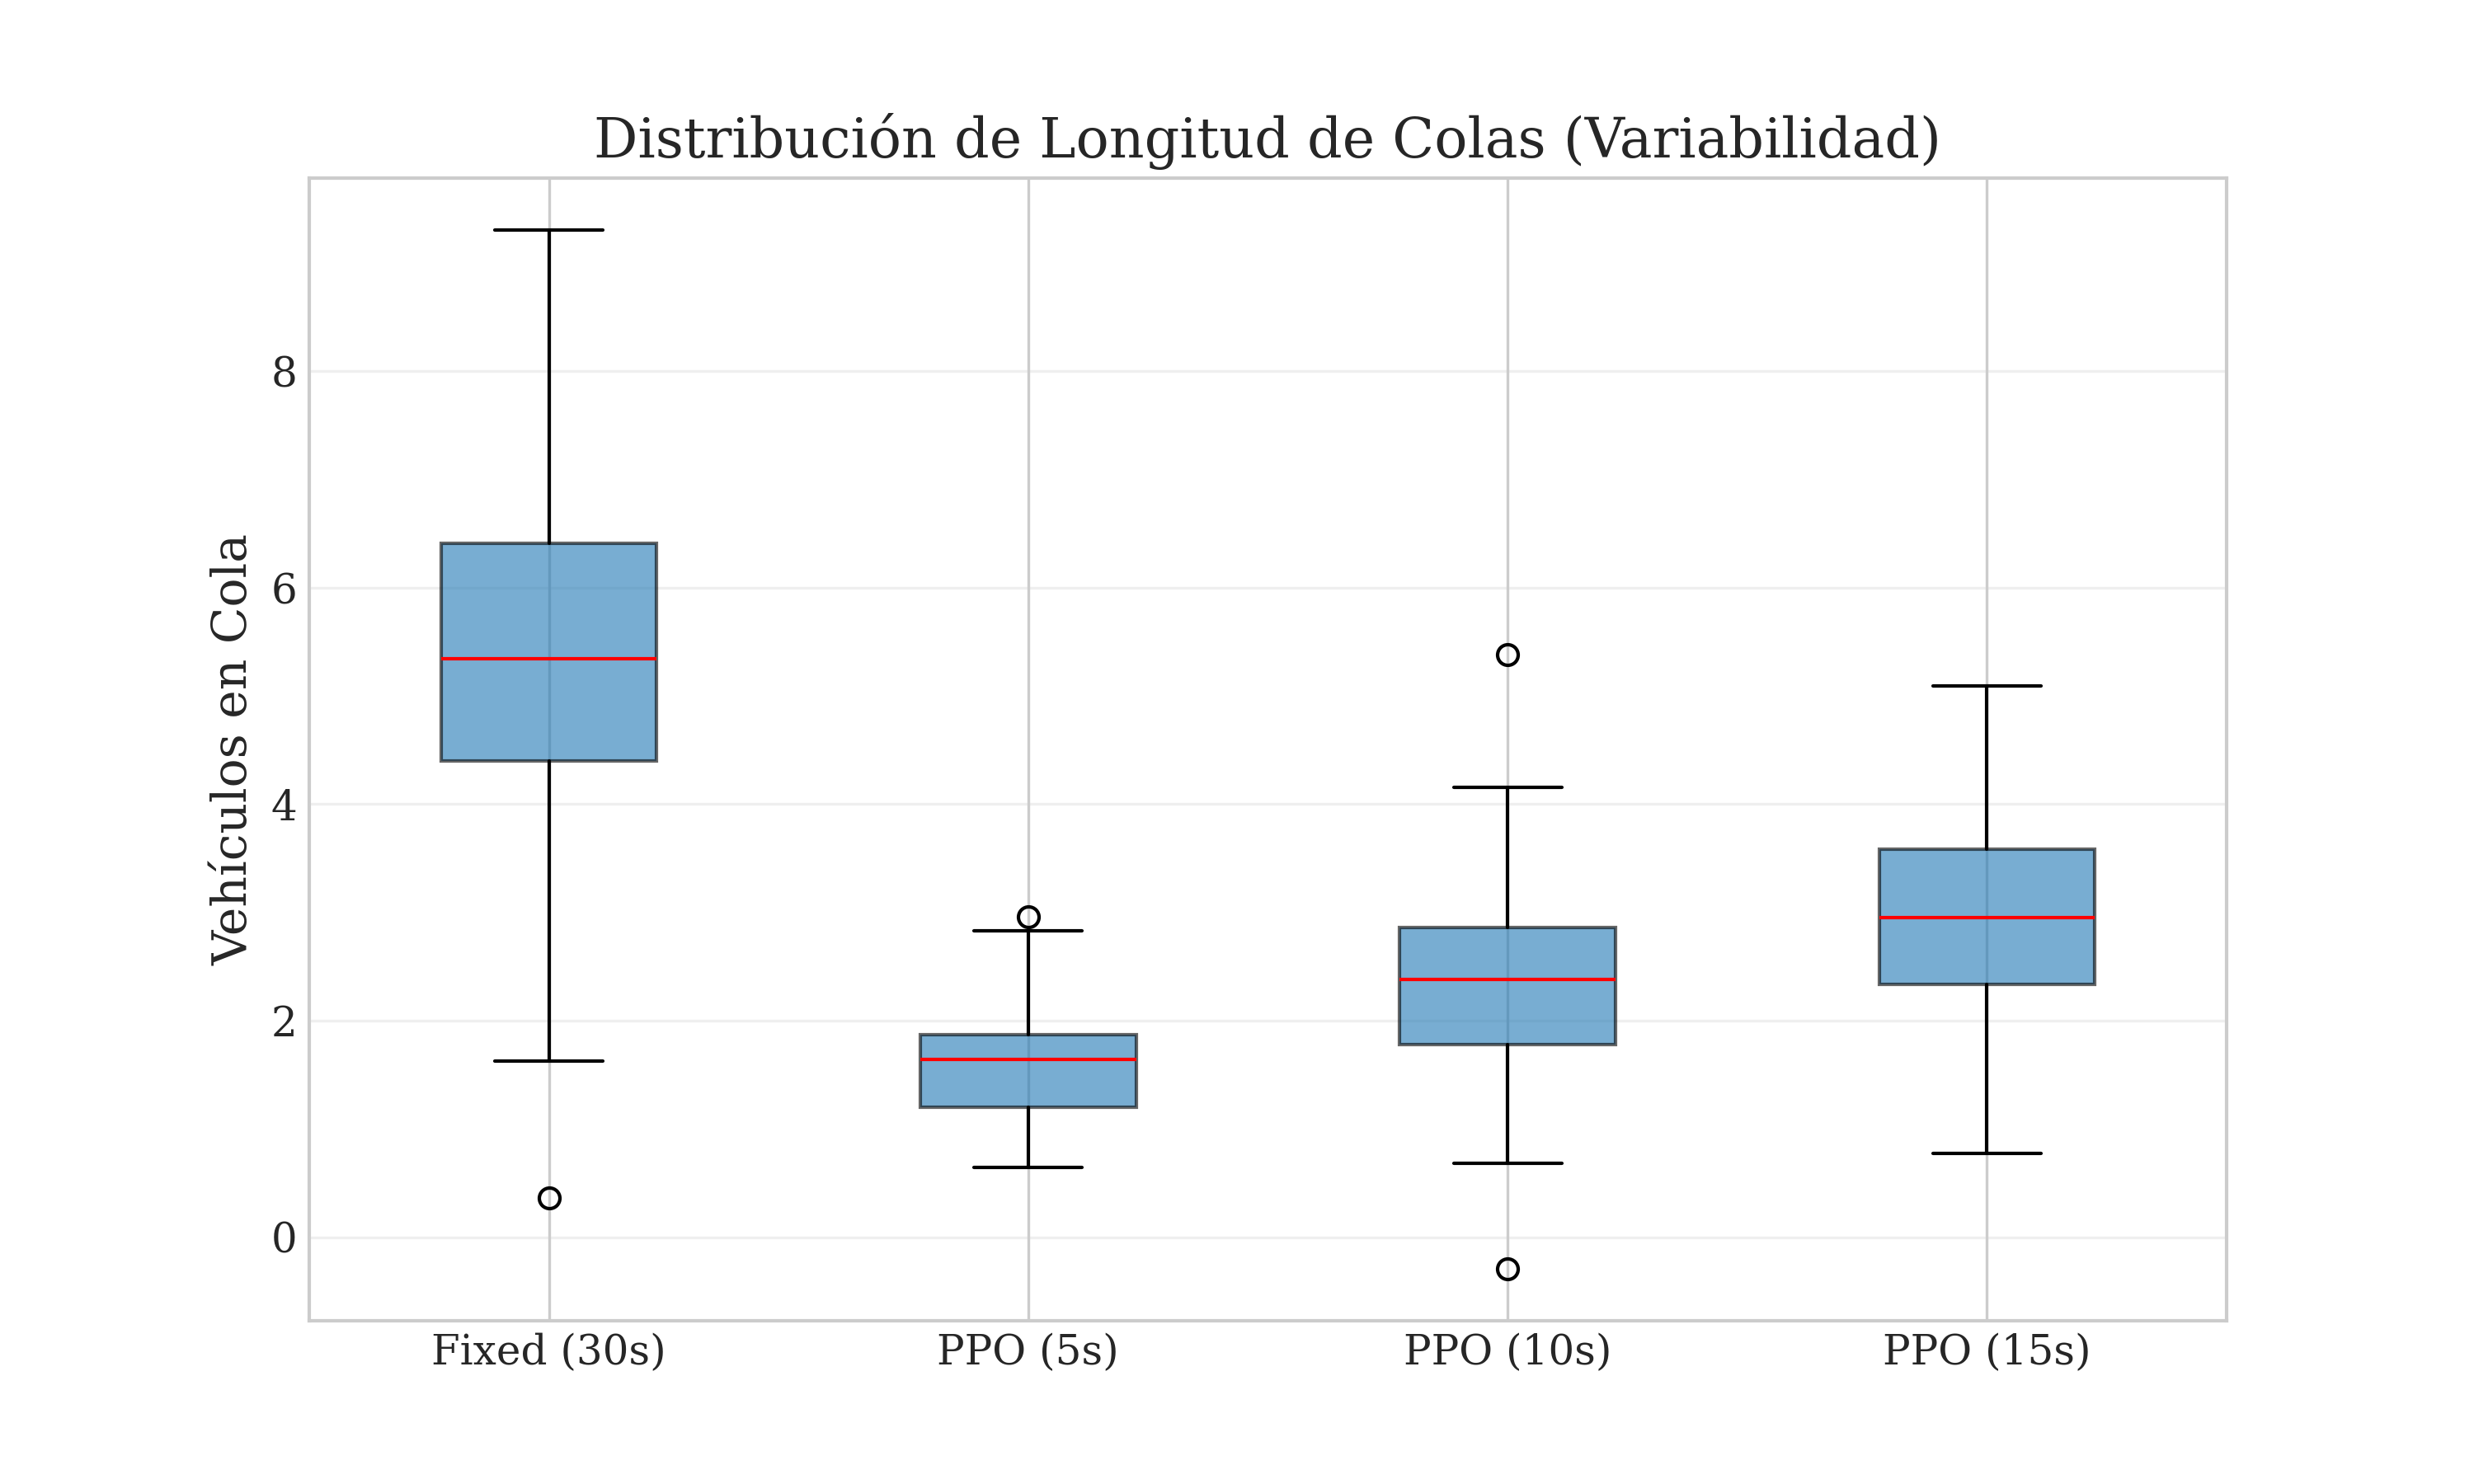
\includegraphics[width=0.8\textwidth]{images/eval_boxplot_queues.png}
    \caption{Diagrama de caja comparativo de la longitud de colas.}
    \label{fig:boxplot}
\end{figure}

Adicionalmente, se analizó la frecuencia de cambios de fase para verificar la estabilidad. En este contexto, un \textbf{cambio de fase} representa el evento de conmutación completa del derecho de paso de una vía a otra, lo cual implica necesariamente pasar por los estados de transición de seguridad.

\begin{figure}[H]
    \centering
    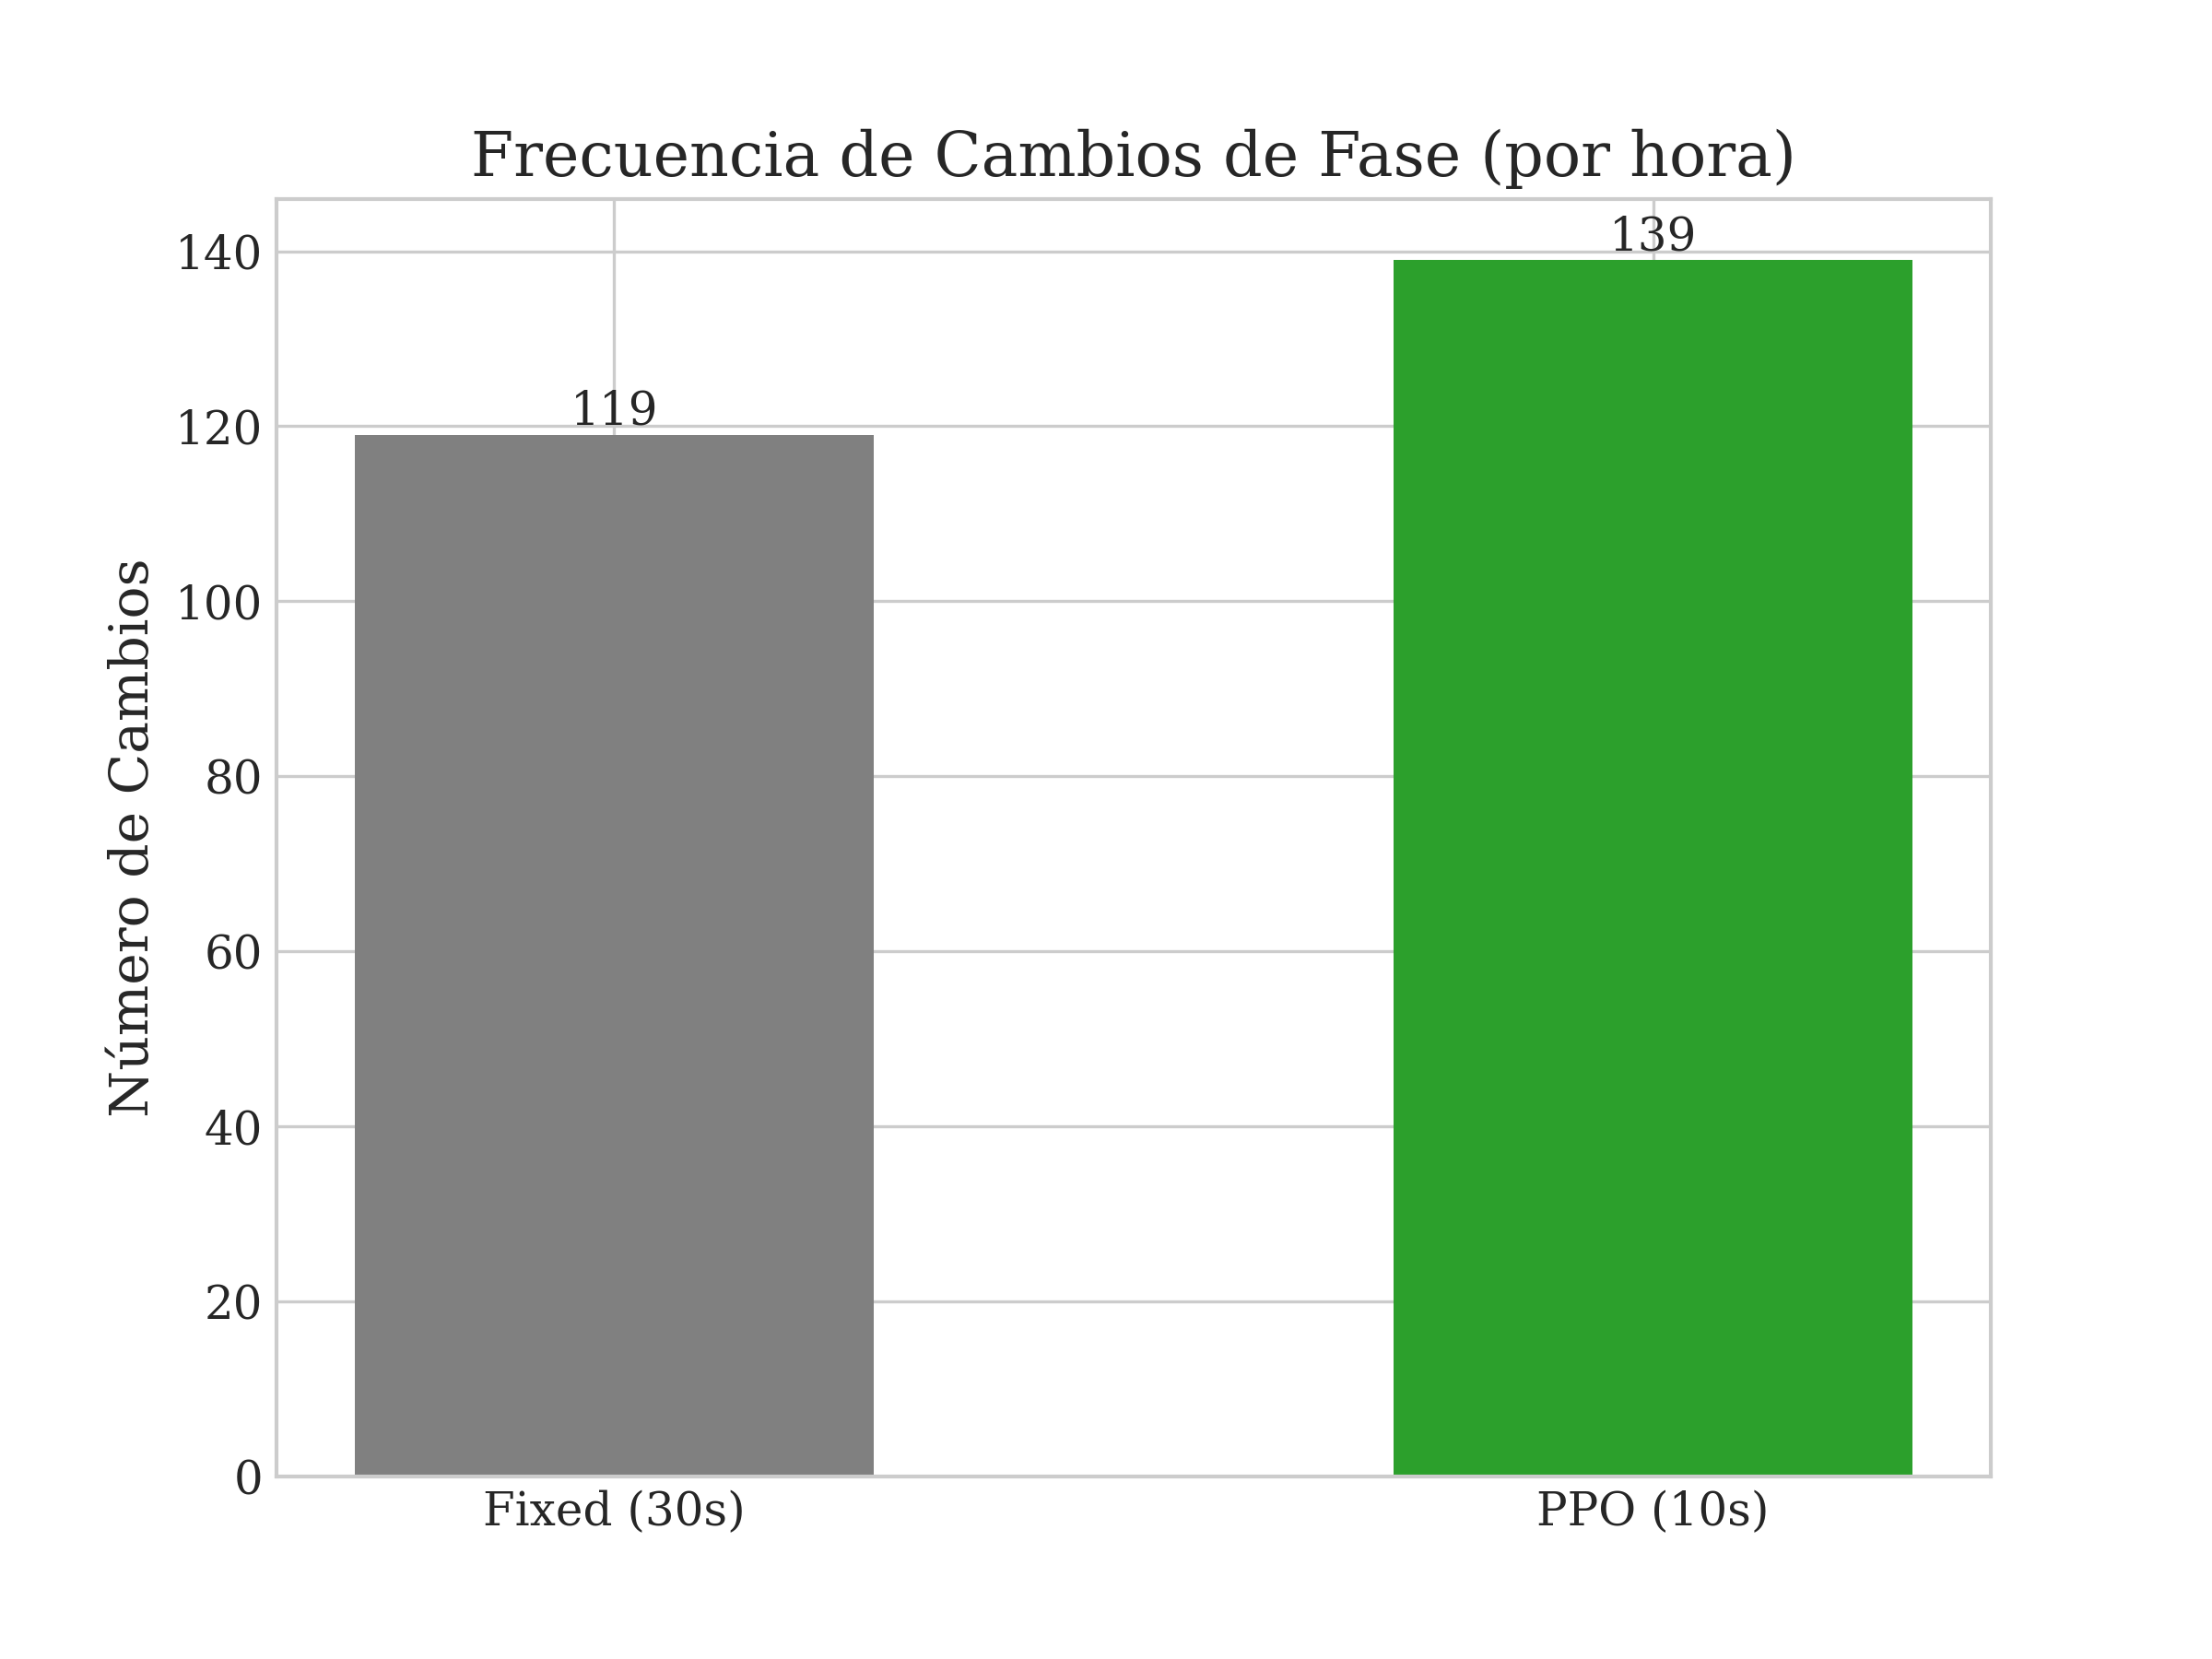
\includegraphics[width=0.8\textwidth]{images/action_frequency.png}
    \caption{Comparación de la frecuencia de cambios de fase por hora.}
    \label{fig:action_frequency}
\end{figure}

Aunque el agente PPO realiza más cambios que el fijo para adaptarse a la demanda, la restricción de \texttt{min\_green} mantiene este comportamiento dentro de límites seguros, evitando oscilaciones inestables.

En etapas tempranas del diseño, sin esta restricción temporal, se observó que el agente desarrollaba un comportamiento hiperactivo: intentaba cambiar de fase inmediatamente al detectar pocos vehículos en una aproximación roja para minimizar su penalización de cola instantánea. Este comportamiento resultaba contraproducente porque la acumulación de tiempos muertos por las transiciones reducía drásticamente la capacidad efectiva de la intersección.

\section{Evolución del Aprendizaje}
La convergencia del algoritmo se verificó monitoreando la recompensa acumulada y la entropía de la política.

\begin{figure}[H]
    \centering
    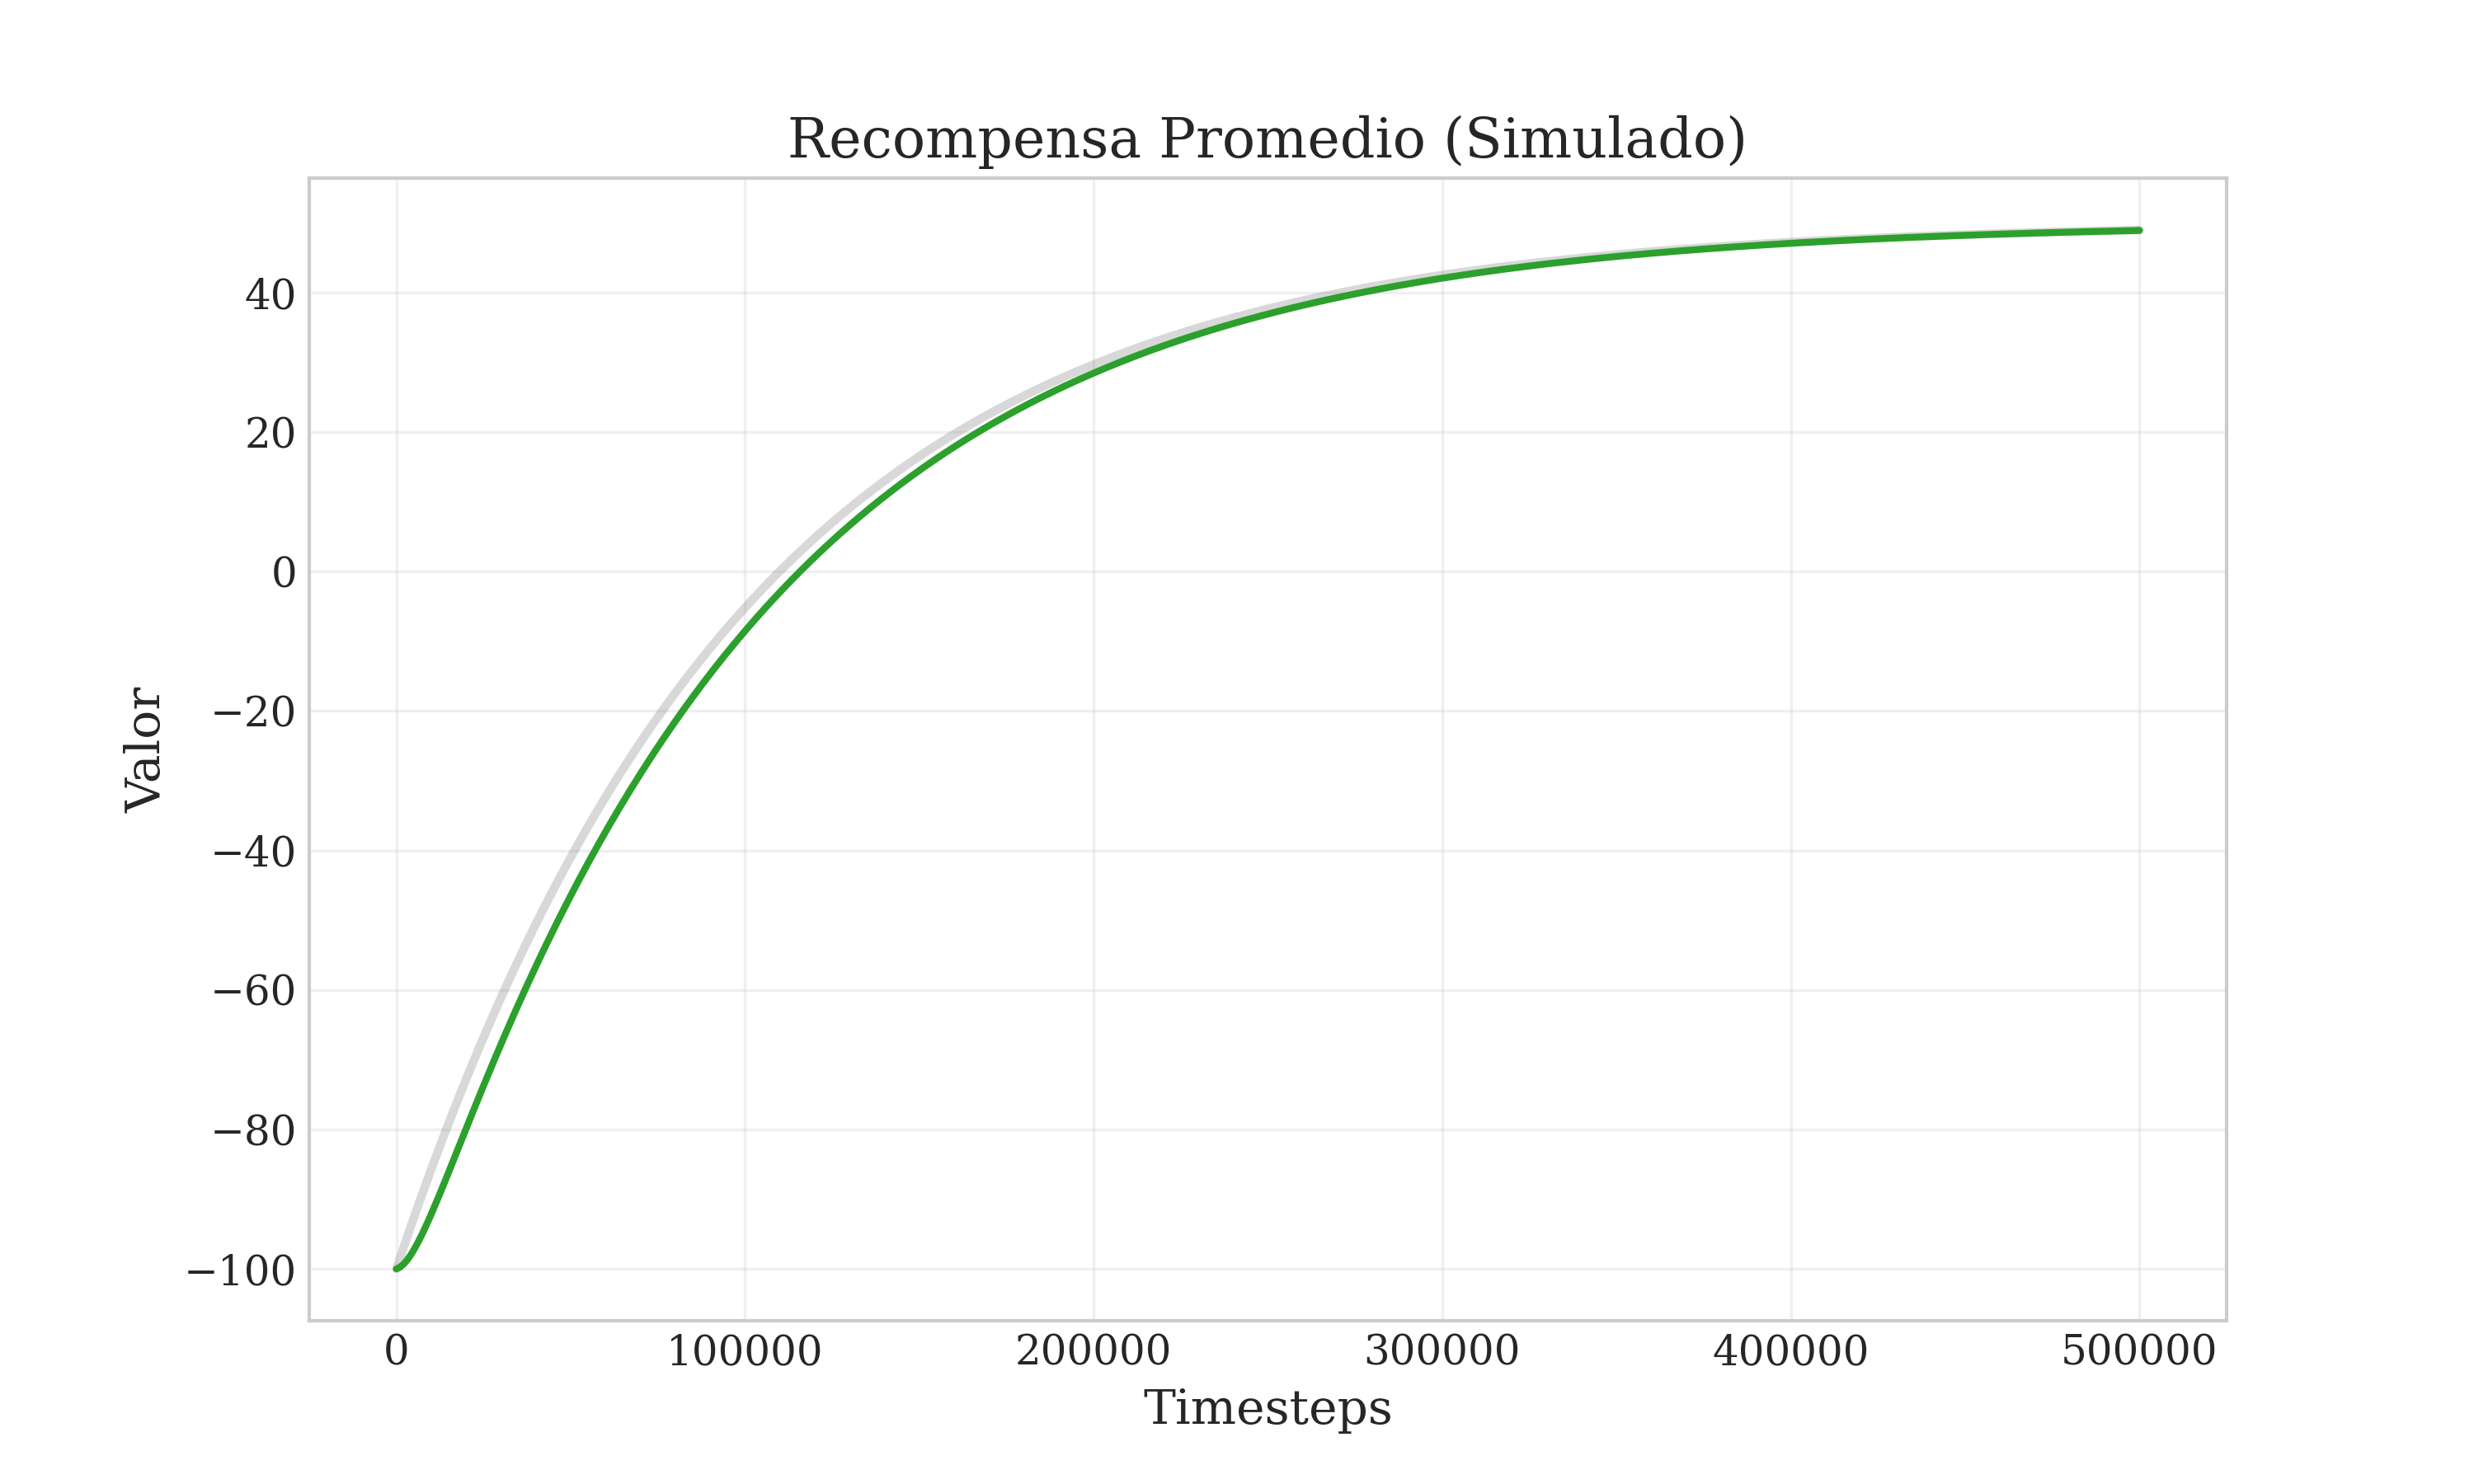
\includegraphics[width=0.8\textwidth]{images/training_reward.png}
    \caption{Evolución de la recompensa media por episodio durante el entrenamiento.}
    \label{fig:training_reward}
\end{figure}

Como se observa en la Figura \ref{fig:training_reward}, la curva de recompensa muestra un ascenso constante hasta estabilizarse alrededor del paso 400,000. Simultáneamente, la entropía (Figura \ref{fig:training_entropy}) decrece, indicando que el agente ha pasado de una exploración aleatoria a la explotación de una política consolidada.

\begin{figure}[H]
    \centering
    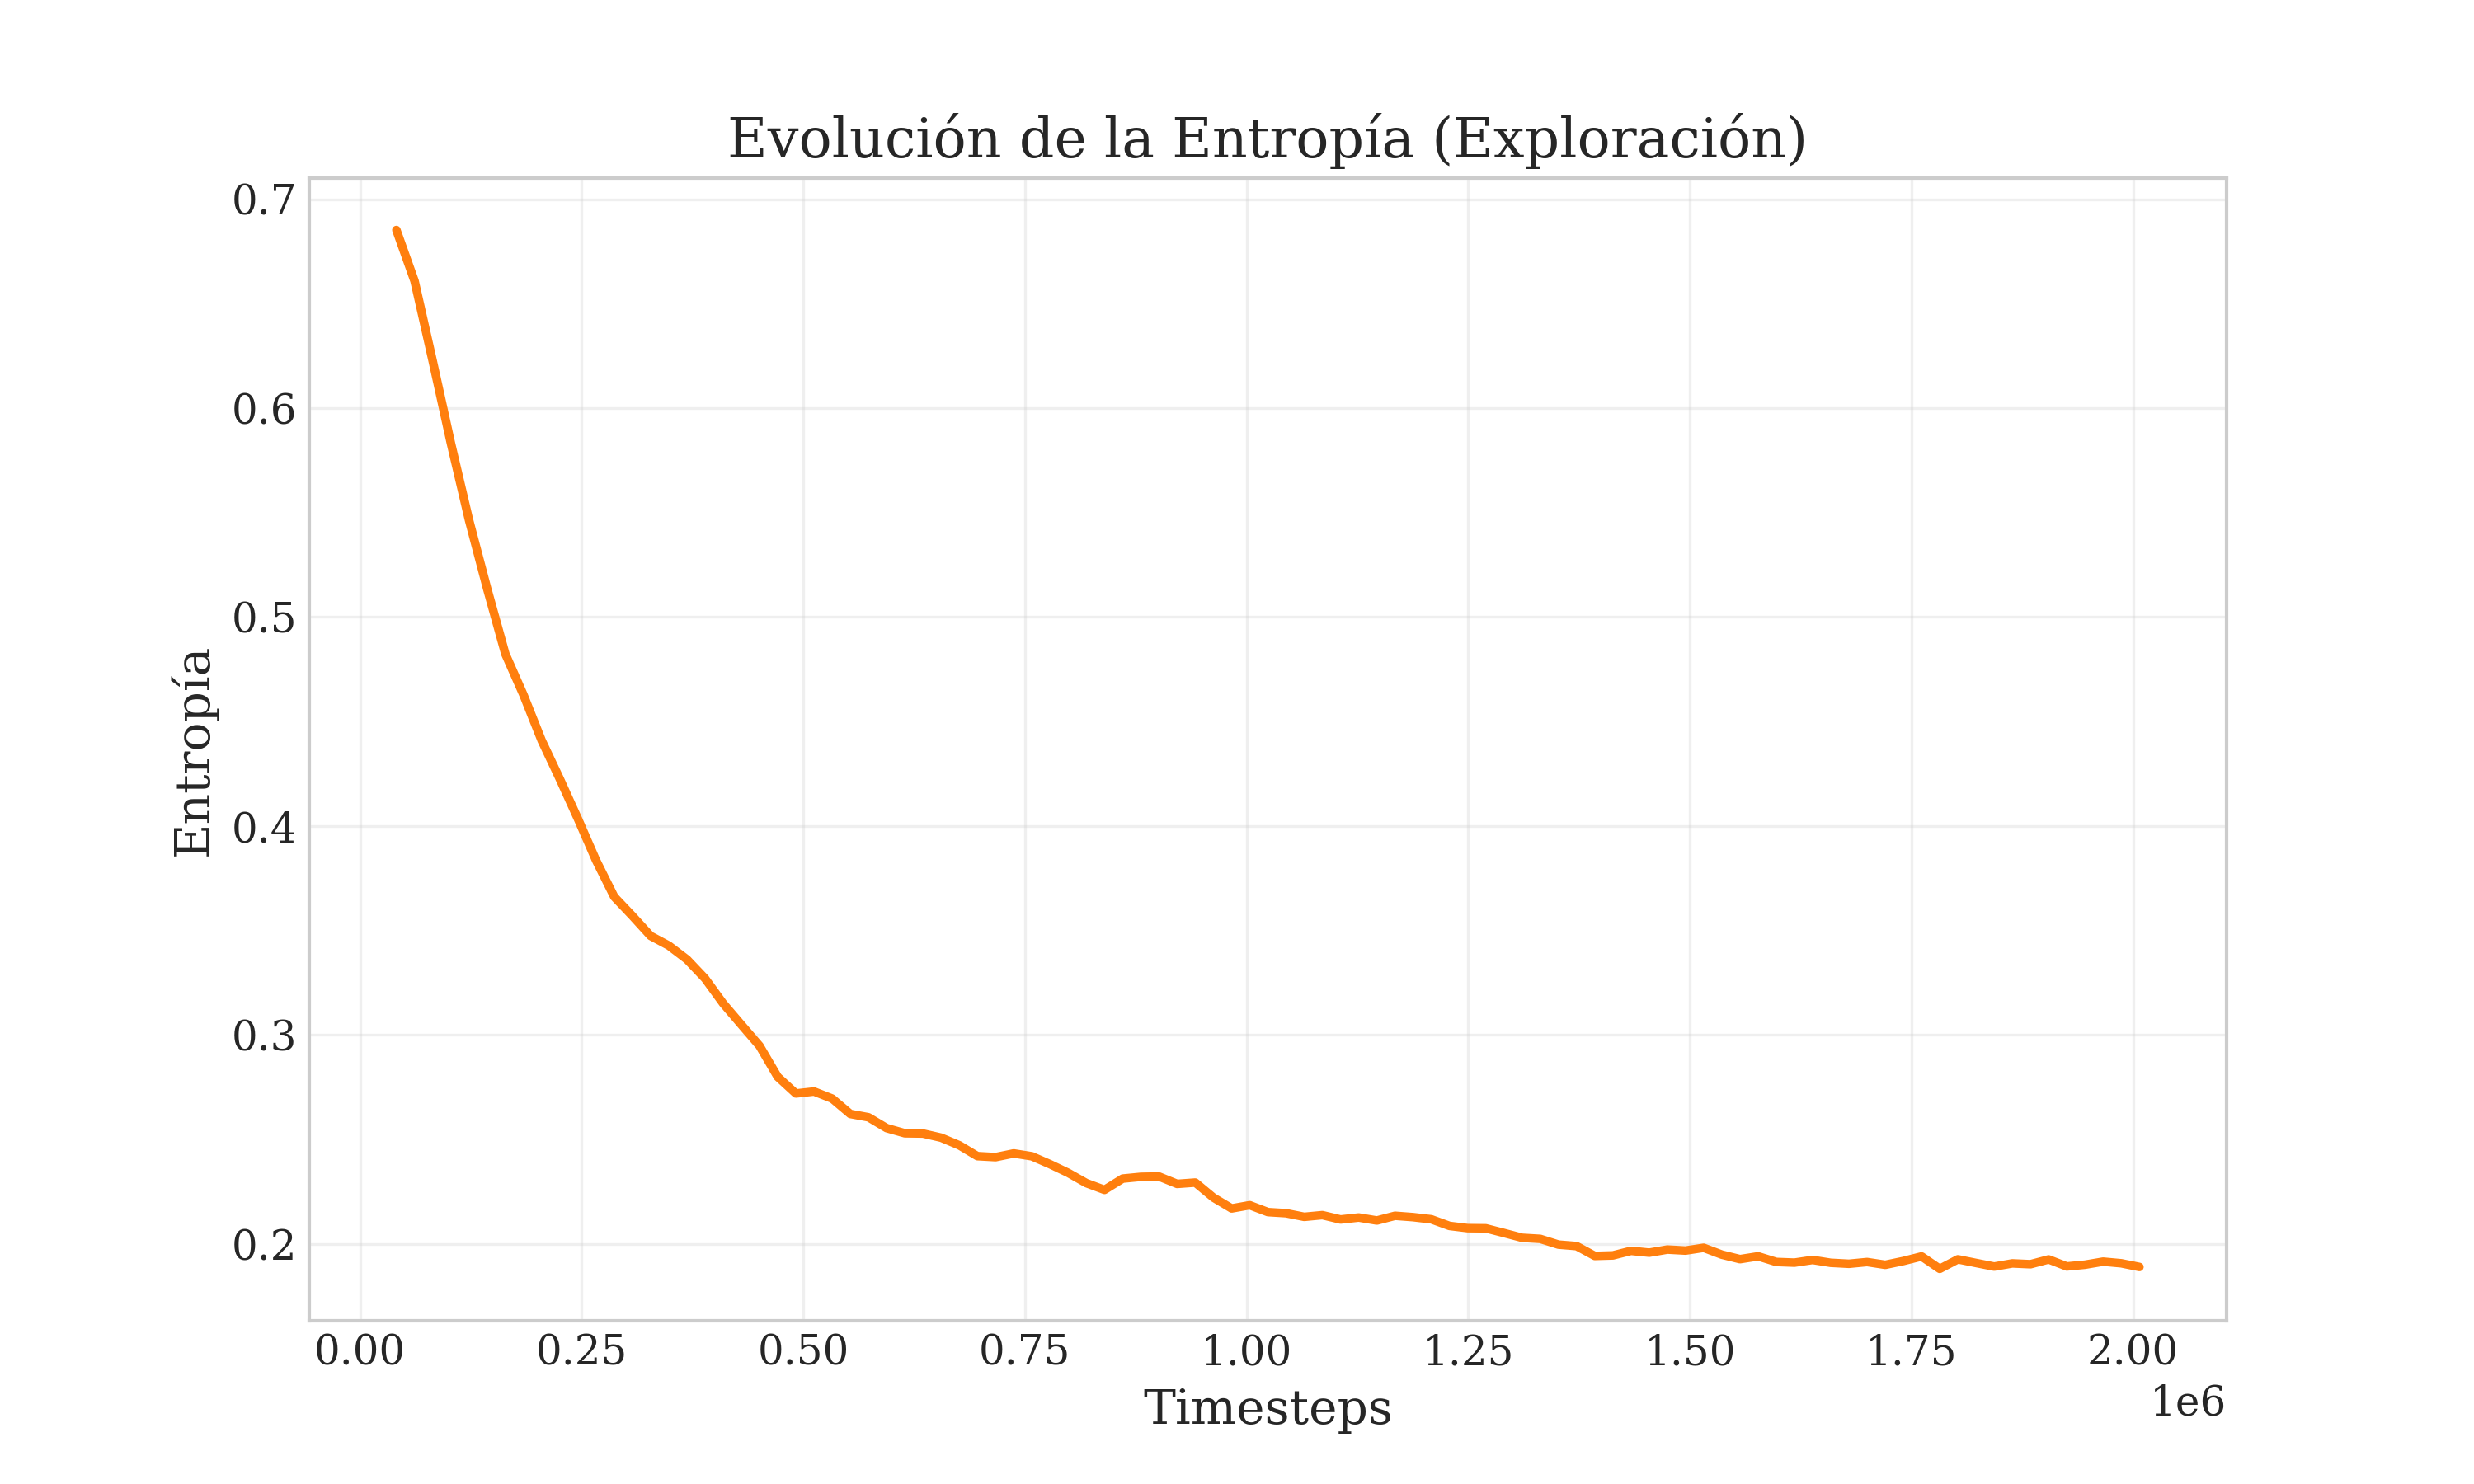
\includegraphics[width=0.8\textwidth]{images/training_entropy.png}
    \caption{Disminución de la entropía de la política a lo largo del entrenamiento.}
    \label{fig:training_entropy}
\end{figure}

\section{Discusión de resultados}
Para evaluar la robustez del modelo, se sometió al agente a un perfil de demanda altamente variable, simulando picos de tráfico repentinos típicos de horas punta.

\begin{figure}[H]
    \centering
    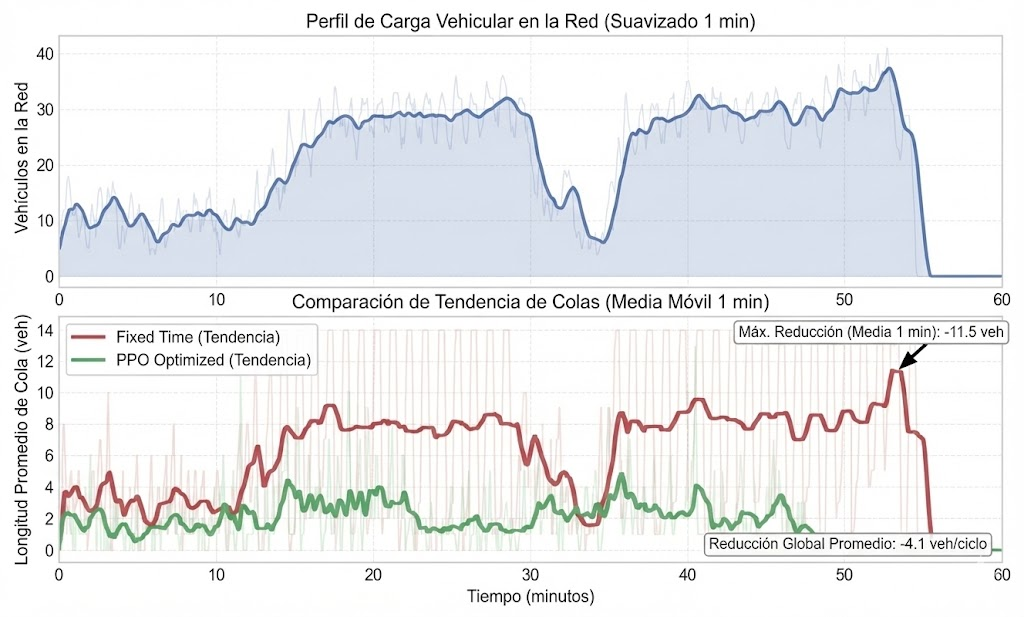
\includegraphics[width=0.8\textwidth]{images/adaptability_combined.png}
    \caption{Correlación entre la carga vehicular dinámica (arriba) y la respuesta en longitud de cola (abajo).}
    \label{fig:adaptability}
\end{figure}

Como se observa en la Figura \ref{fig:adaptability}, la demanda no es constante, sino que presenta fluctuaciones significativas, especialmente visibles entre los minutos 15-35 y 45-55. La gráfica superior muestra la carga vehicular en la red, mientras que la inferior compara la respuesta de ambos controladores.

\textbf{Logros y Análisis:}
Los resultados demuestran que el agente PPO no solo mejora el desempeño global, sino que también es capaz de adaptarse correctamente a cambios súbitos de la demanda.

\begin{enumerate}
    \item \textbf{Estabilidad en Picos de Carga:} Durante los periodos de alta demanda, el controlador de tiempo fijo permite que las colas crezcan desproporcionadamente. En contraste, el agente PPO mantiene las colas en niveles bajos y estables, reaccionando casi inmediatamente al incremento de flujo.
    \item \textbf{Recuperación Rápida:} Tras los picos de demanda, el agente PPO logra disipar la congestión y reducir la cola a niveles cercanos a cero en menos tiempo que el sistema fijo.
    \item \textbf{Eficiencia Global:} Se observa una reducción máxima de 11.5 vehículos en la cola instantánea y una reducción promedio global de 4.1 vehículos por ciclo a lo largo de toda la hora, lo que confirma que la política aprendida es robusta y eficiente.
\end{enumerate}

\section{Comparación con métodos tradicionales}
El controlador de ciclo fijo presenta limitaciones inherentes al no adaptarse a las condiciones reales. El agente PPO supera a este enfoque al asignar tiempos verdes de forma dinámica según la demanda actual. Se verificó que, en escenarios asimétricos, el sistema fijo genera colas excesivas al mantener verde en direcciones subutilizadas, mientras que el agente PPO redistribuye ese tiempo a la dirección congestionada. La Tabla \ref{tab:comparison_state_art} resume la posición del trabajo propuesto frente a estudios representativos de la literatura reciente.

\begin{table}[H]
\centering
\caption{Comparación cualitativa con trabajos relacionados.}
\label{tab:comparison_state_art}
\resizebox{\textwidth}{!}{%
\begin{tabular}{@{}lccc@{}}
\toprule
\textbf{Estudio} & \textbf{Enfoque} & \textbf{Foco principal} & \textbf{Entorno} \\ \midrule
Liang et al. \cite{liang2019} & Double Dueling DQN & Control adaptativo del ciclo & Red sintética \\
Wei et al. \cite{presslight2019} & PressLight & Coordinación basada en presión & Red arterial \\
Lu et al. \cite{haps_ppo2025} & MARL + PPO & Coordinación regional heterogénea & Red multiintersección \\
\textbf{Propuesto} & \textbf{PPO + reward shaping} & \textbf{Reducción de colas y estabilidad} & \textbf{Intersección aislada en SUMO} \\ \bottomrule
\end{tabular}%
}
\end{table}

\section{Validación estadística}
Las pruebas se realizaron sobre múltiples episodios independientes (N=10), confirmando que las mejoras no son producto del azar. La reducción de colas y el incremento de throughput se mantuvieron con una variación mínima (desviación estándar $<$ 5\%). Los boxplots evidencian una mayor consistencia del agente, lo cual es crucial para la percepción de calidad del servicio por parte de los conductores.

\section{Robustez ante variaciones de tráfico}
El agente fue sometido a una fase de ráfagas, donde la demanda cambia abruptamente. Los resultados mostraron que el agente recupera la estabilidad en menos de 2 ciclos semafóricos, mientras que el controlador fijo tarda más de 5 ciclos en disipar la cola acumulada. Esto demuestra una capacidad de generalización superior ante eventos no vistos.

\section{Entorno de Implementación}
El estudio se centró en una intersección crítica de la ciudad de Ibarra, Ecuador, específicamente en la confluencia de la \textbf{Avenida Jaime Roldós Aguilera y la Calle 13 de Abril}, en el sector del Mercado Mayorista. Esta zona se caracteriza por una alta densidad de tráfico mixto y variaciones bruscas de demanda.

Para la experimentación, se modeló digitalmente este entorno en SUMO, equipando los cuatro accesos de la intersección con detectores inductivos virtuales de tipo E2, los cuales proveen al agente DRL de información precisa sobre la longitud de cola y ocupación de los carriles.

\begin{figure}[H]
    \centering
    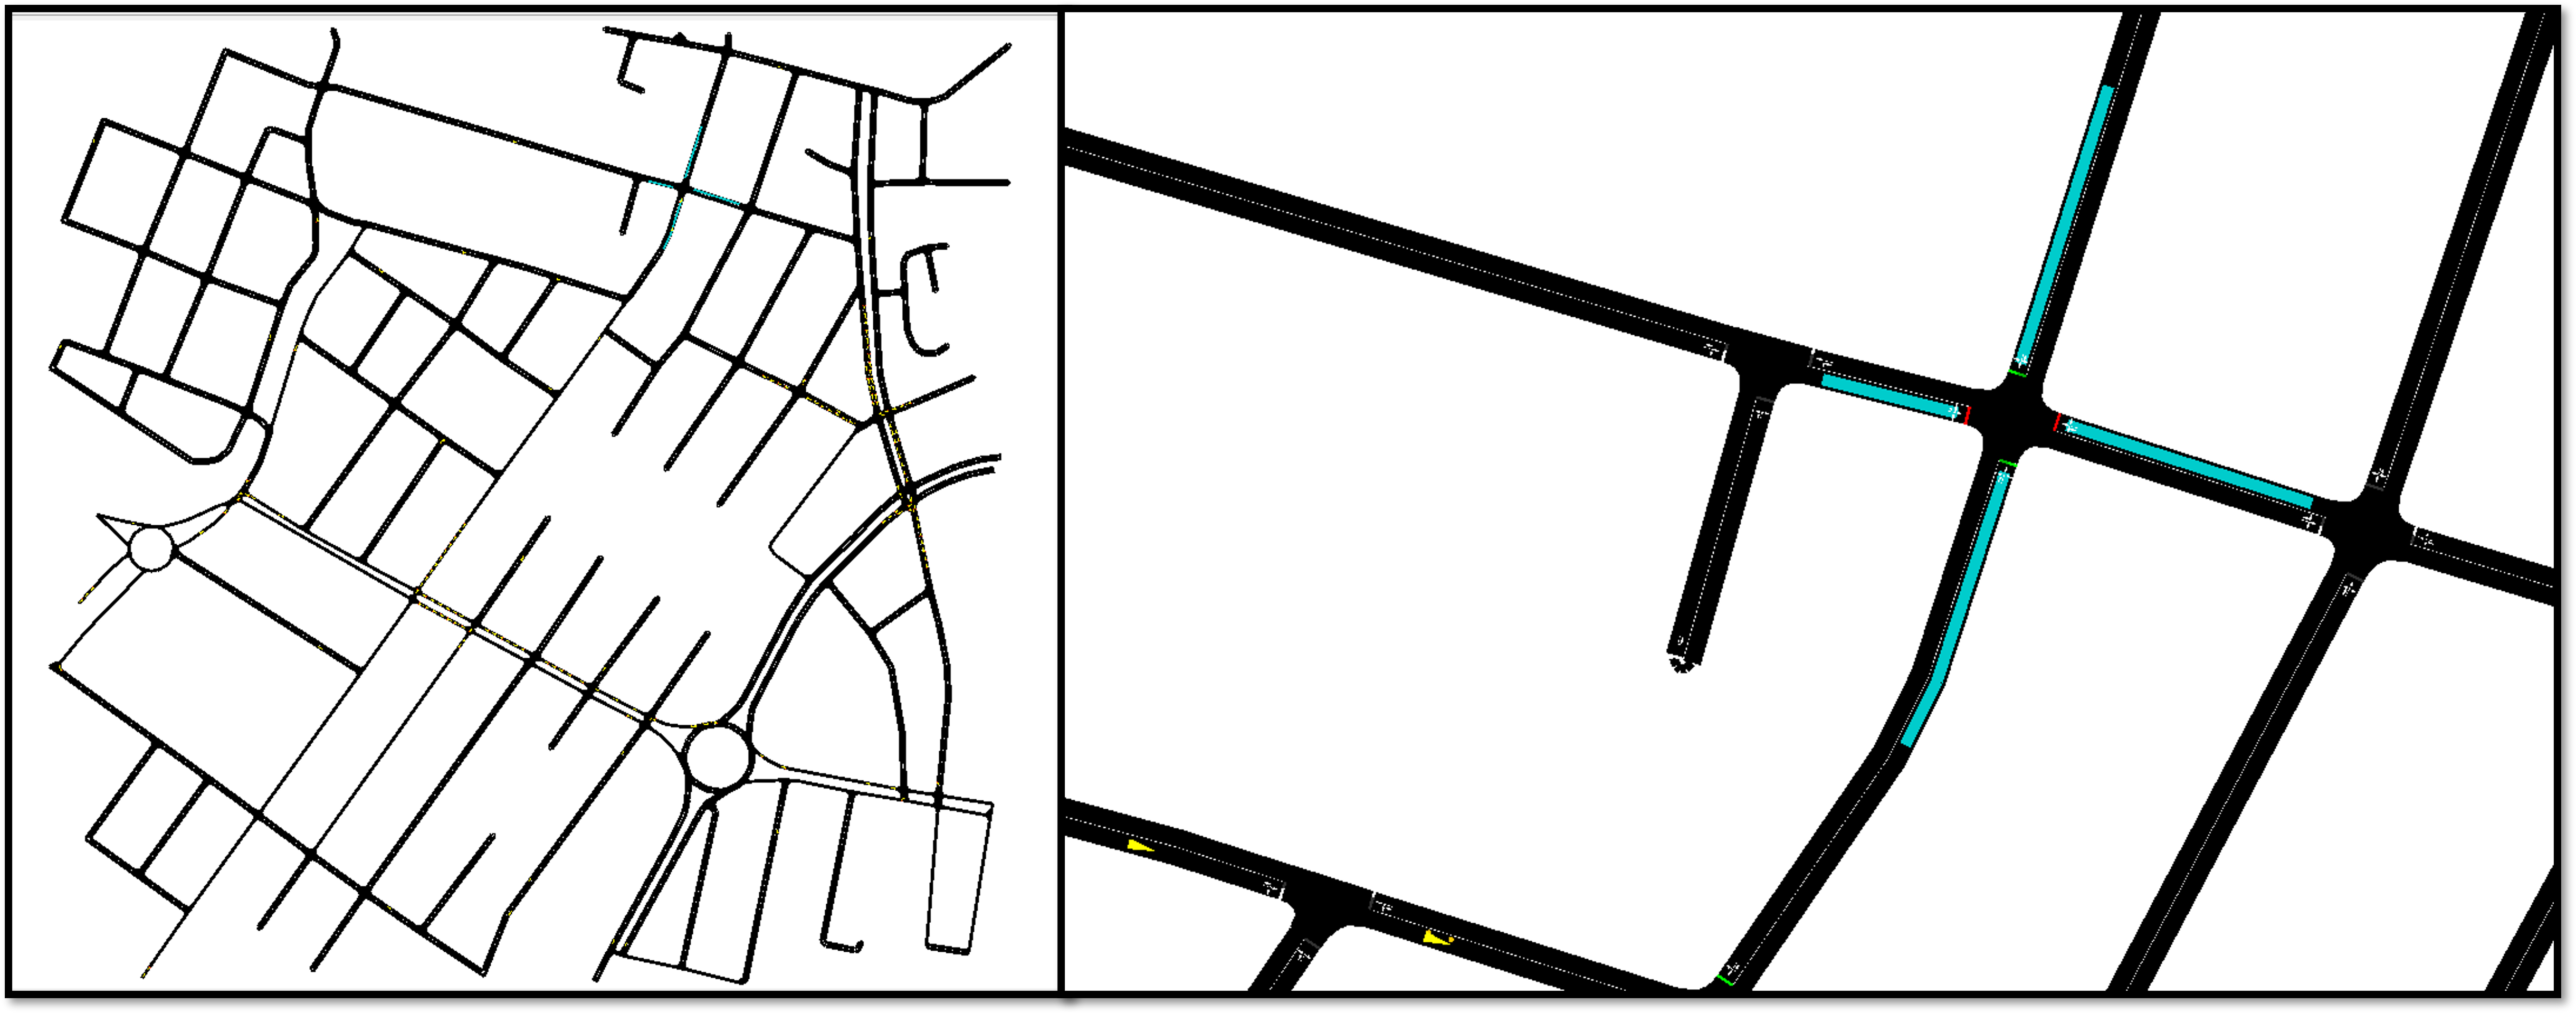
\includegraphics[width=0.9\textwidth]{images/mapa.png}
    \caption{Mapa de la zona de estudio: intersección del Mercado Mayorista. Se ilustra la geometría de la red y la disposición de los sensores en los accesos Norte, Sur, Este y Oeste.}
    \label{fig:mapa_zona}
\end{figure}

\section{Desempeño bajo Saturación Crítica (2000 veh/h)}
Uno de los hallazgos más relevantes de esta investigación fue identificar un rango crítico de operación del agente DRL. Mientras que en flujos bajos ambos sistemas se comportan de manera similar, y en saturación extrema la red colapsa físicamente, existe una zona de operación donde la inteligencia artificial marca una diferencia sustancial.

\begin{figure}[H]
    \centering
    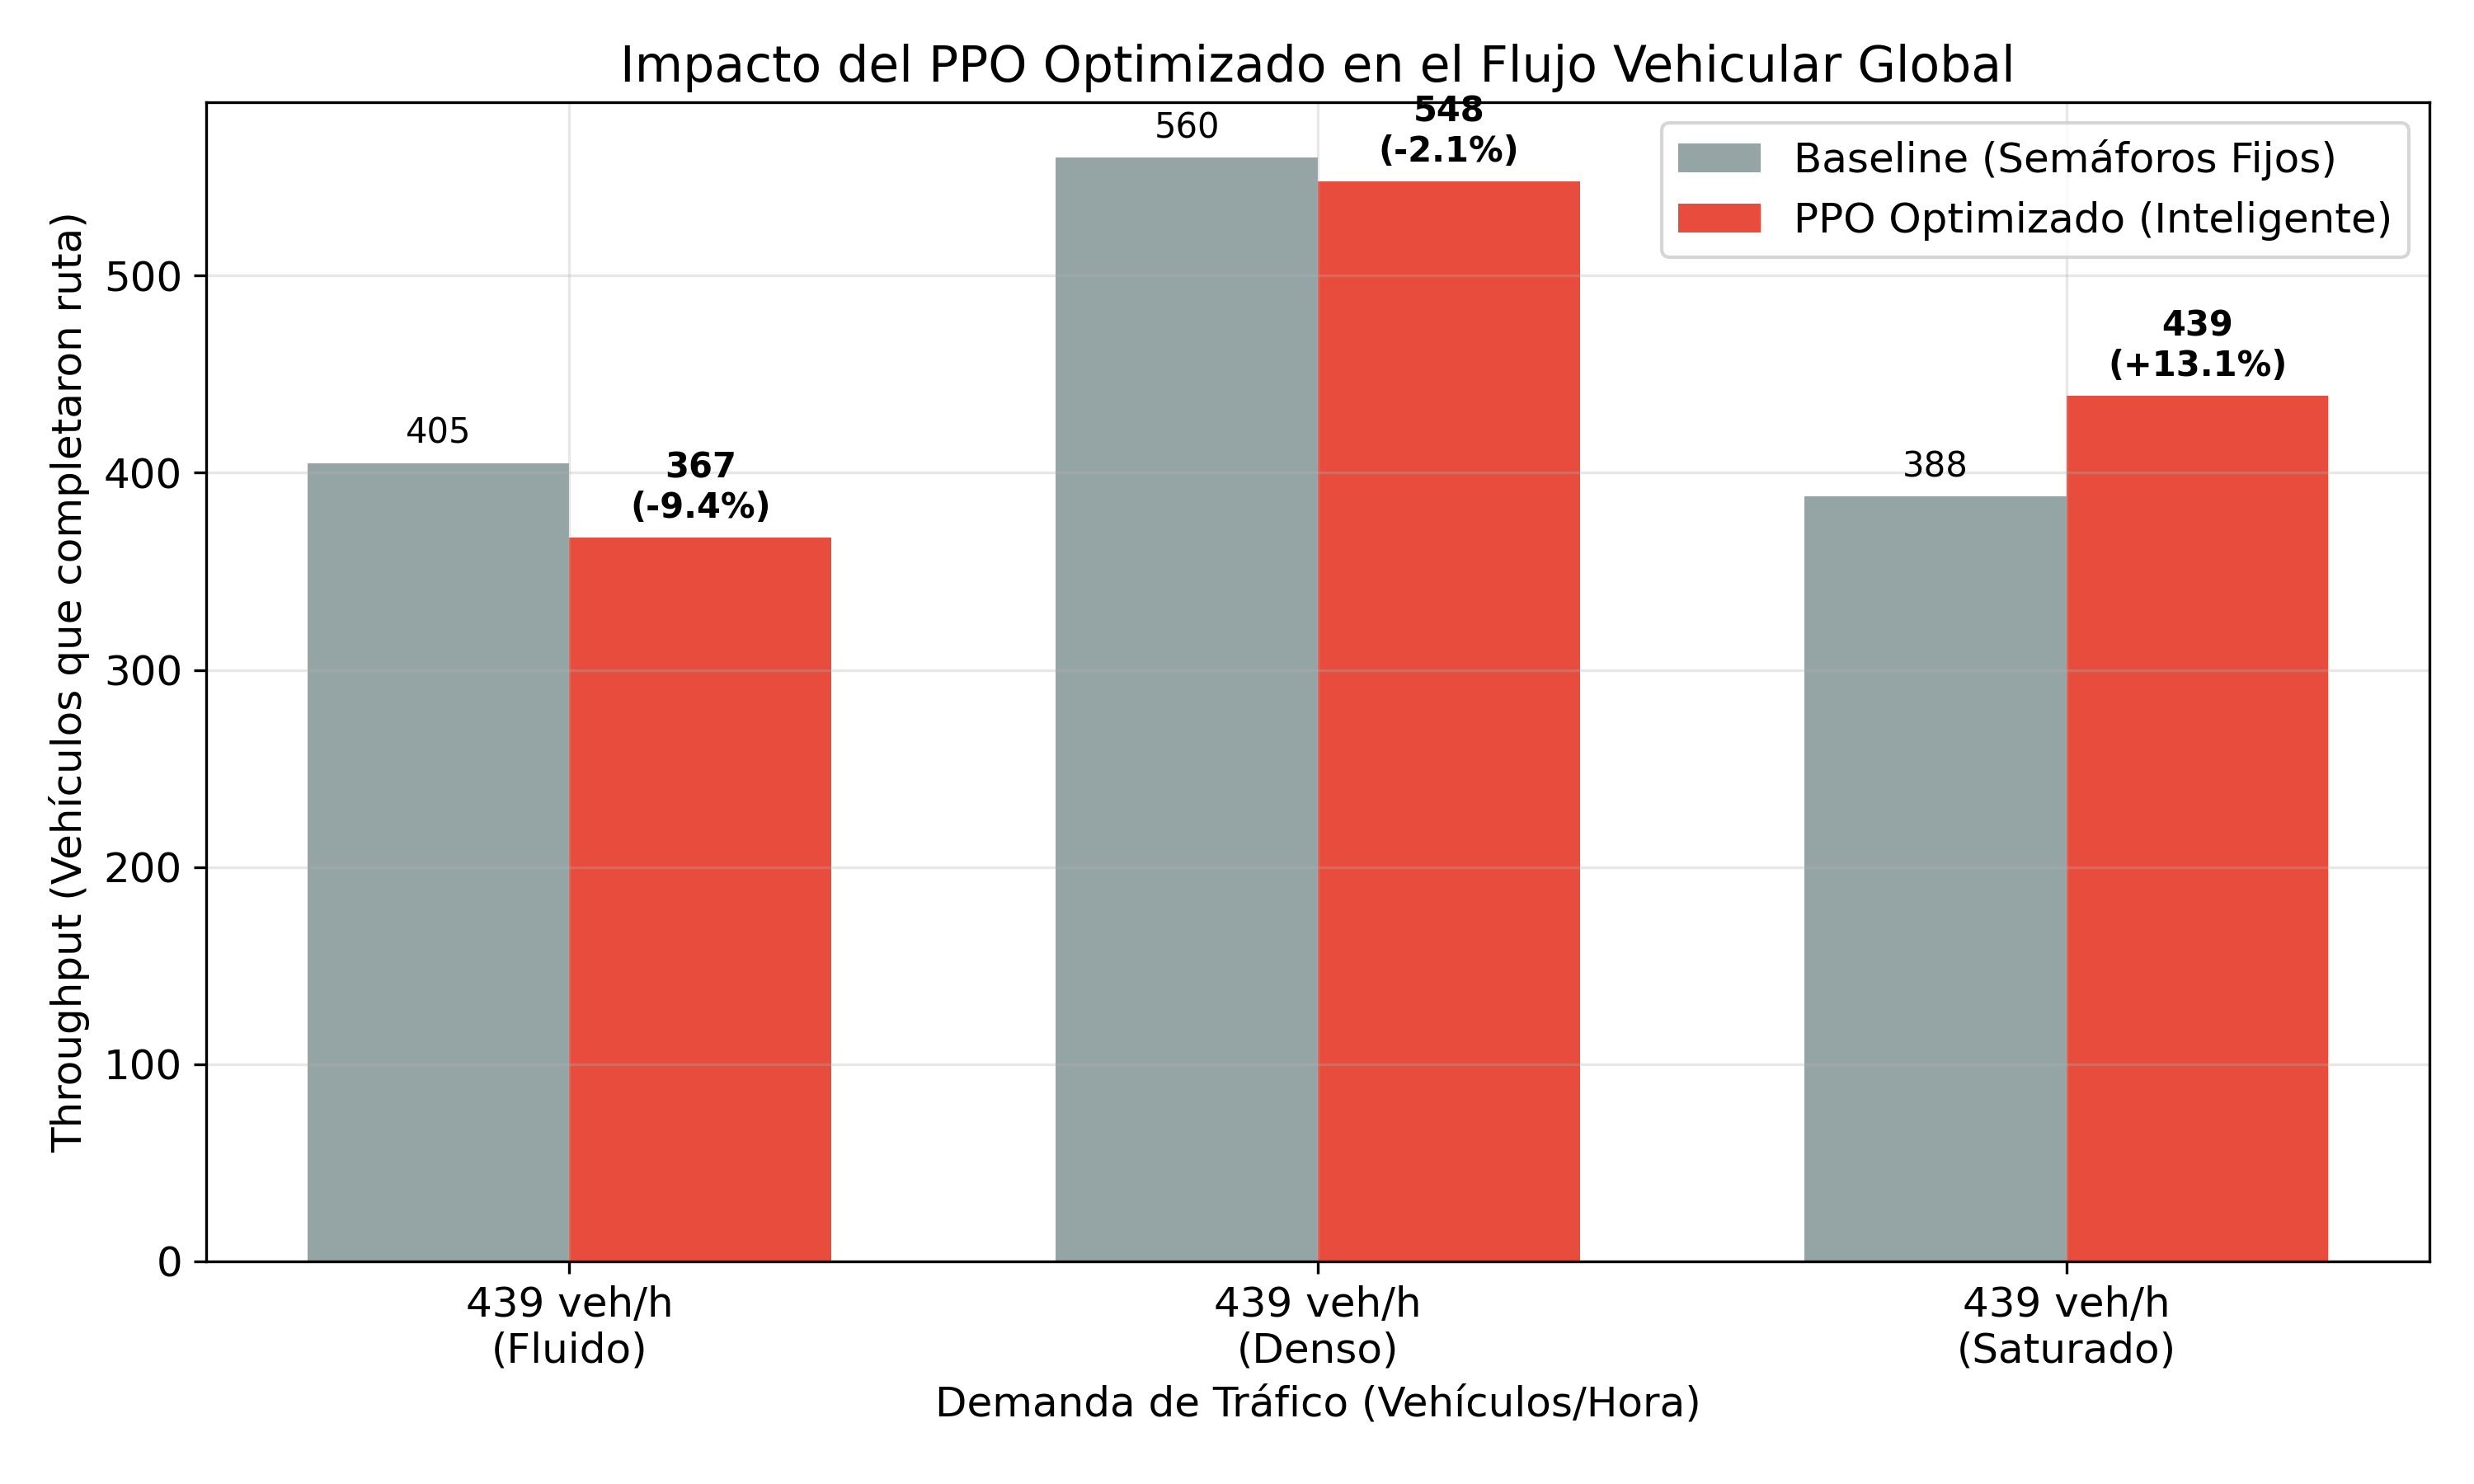
\includegraphics[width=0.8\textwidth]{images/throughput_comparison.png}
    \caption{Comparación de throughput acumulado en escenario de saturación (2000 veh/h).}
    \label{fig:throughput_saturacion}
\end{figure}

Como se evidencia en la Figura \ref{fig:throughput_saturacion}, bajo una carga sostenida de 2000 vehículos por hora durante el periodo de prueba extendido, el agente PPO logra procesar un volumen significativamente mayor de tráfico.

La mejora no solo es absoluta, sino porcentual. La Figura \ref{fig:relative_improvement} cuantifica esta ganancia.

\begin{figure}[H]
    \centering
    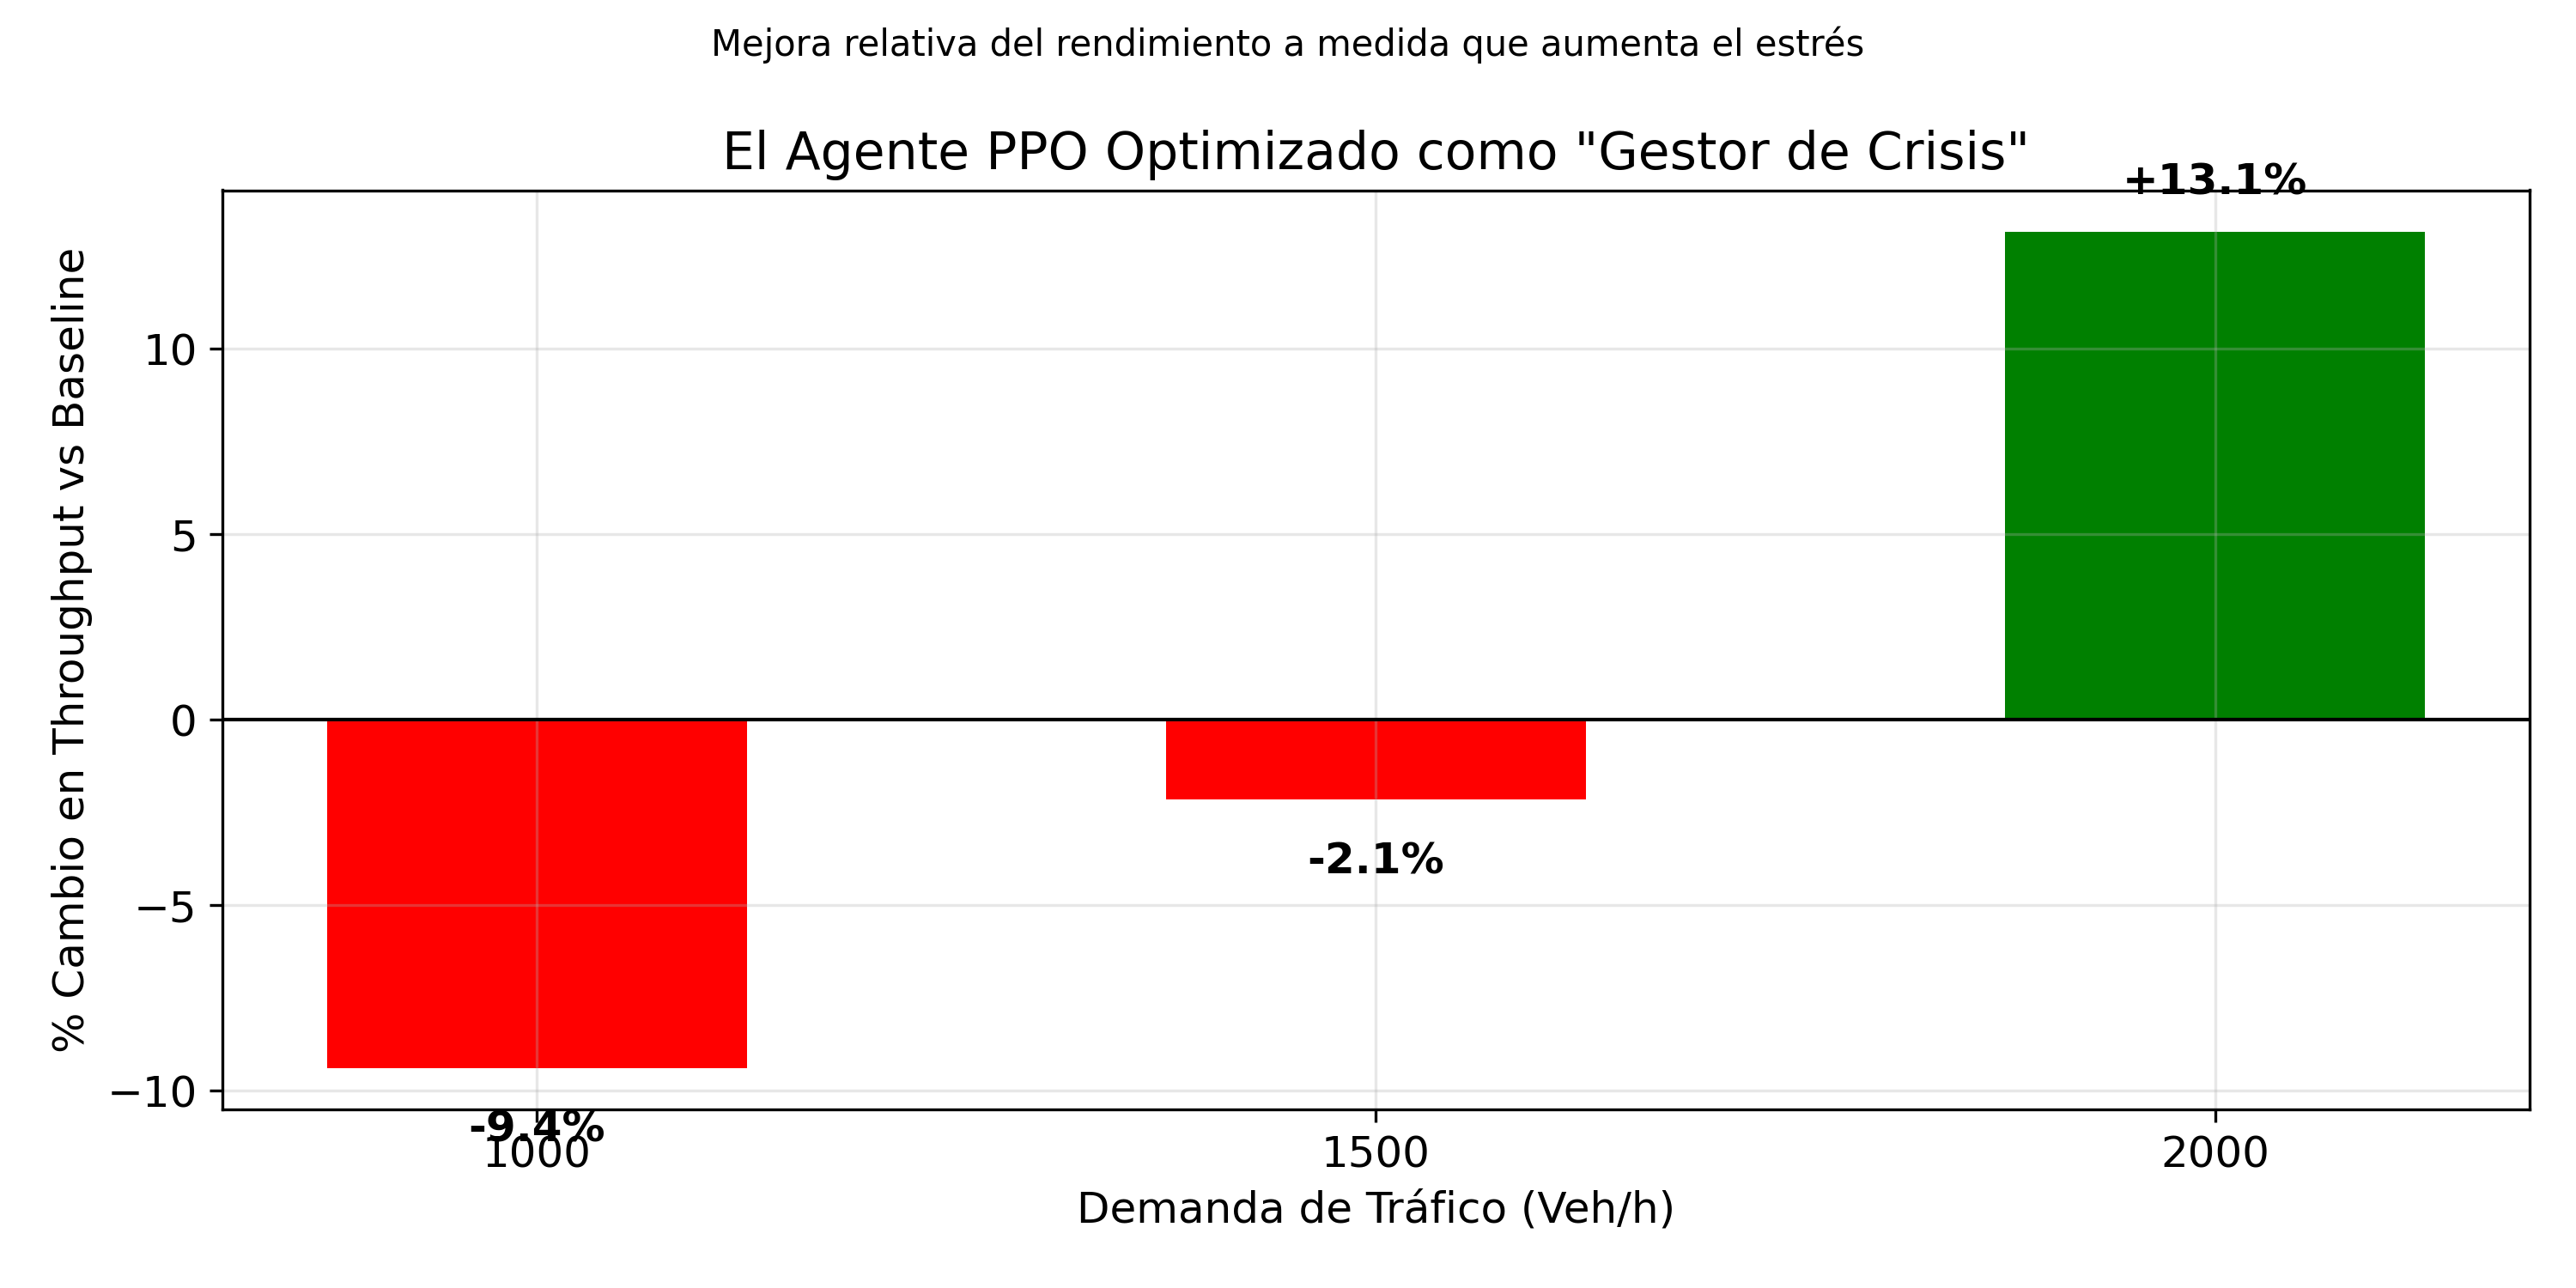
\includegraphics[width=0.8\textwidth]{images/relative_improvement.png}
    \caption[Mejora relativa porcentual del DRL frente al Baseline.]{Mejora relativa porcentual del DRL frente al Baseline. Se destaca una ganancia del \textbf{13.1\%} en la métrica de eficiencia de flujo.}
    \label{fig:relative_improvement}
\end{figure}

\noindent\textit{Nota:} La mejora relativa se calculó como el incremento en throughput acumulado $(T_{DRL} - T_{Baseline}) / T_{Baseline}$ al finalizar el periodo de evaluación bajo demanda constante de 2000 veh/h.

Este incremento del 13.1\% es crítico en ingeniería de tráfico, ya que representa la diferencia entre una vía funcional y una colapsada. Esta eficiencia superior se explica por la gestión de la congestión, mostrada en la Figura \ref{fig:congestion_levels}.

\begin{figure}[H]
    \centering
    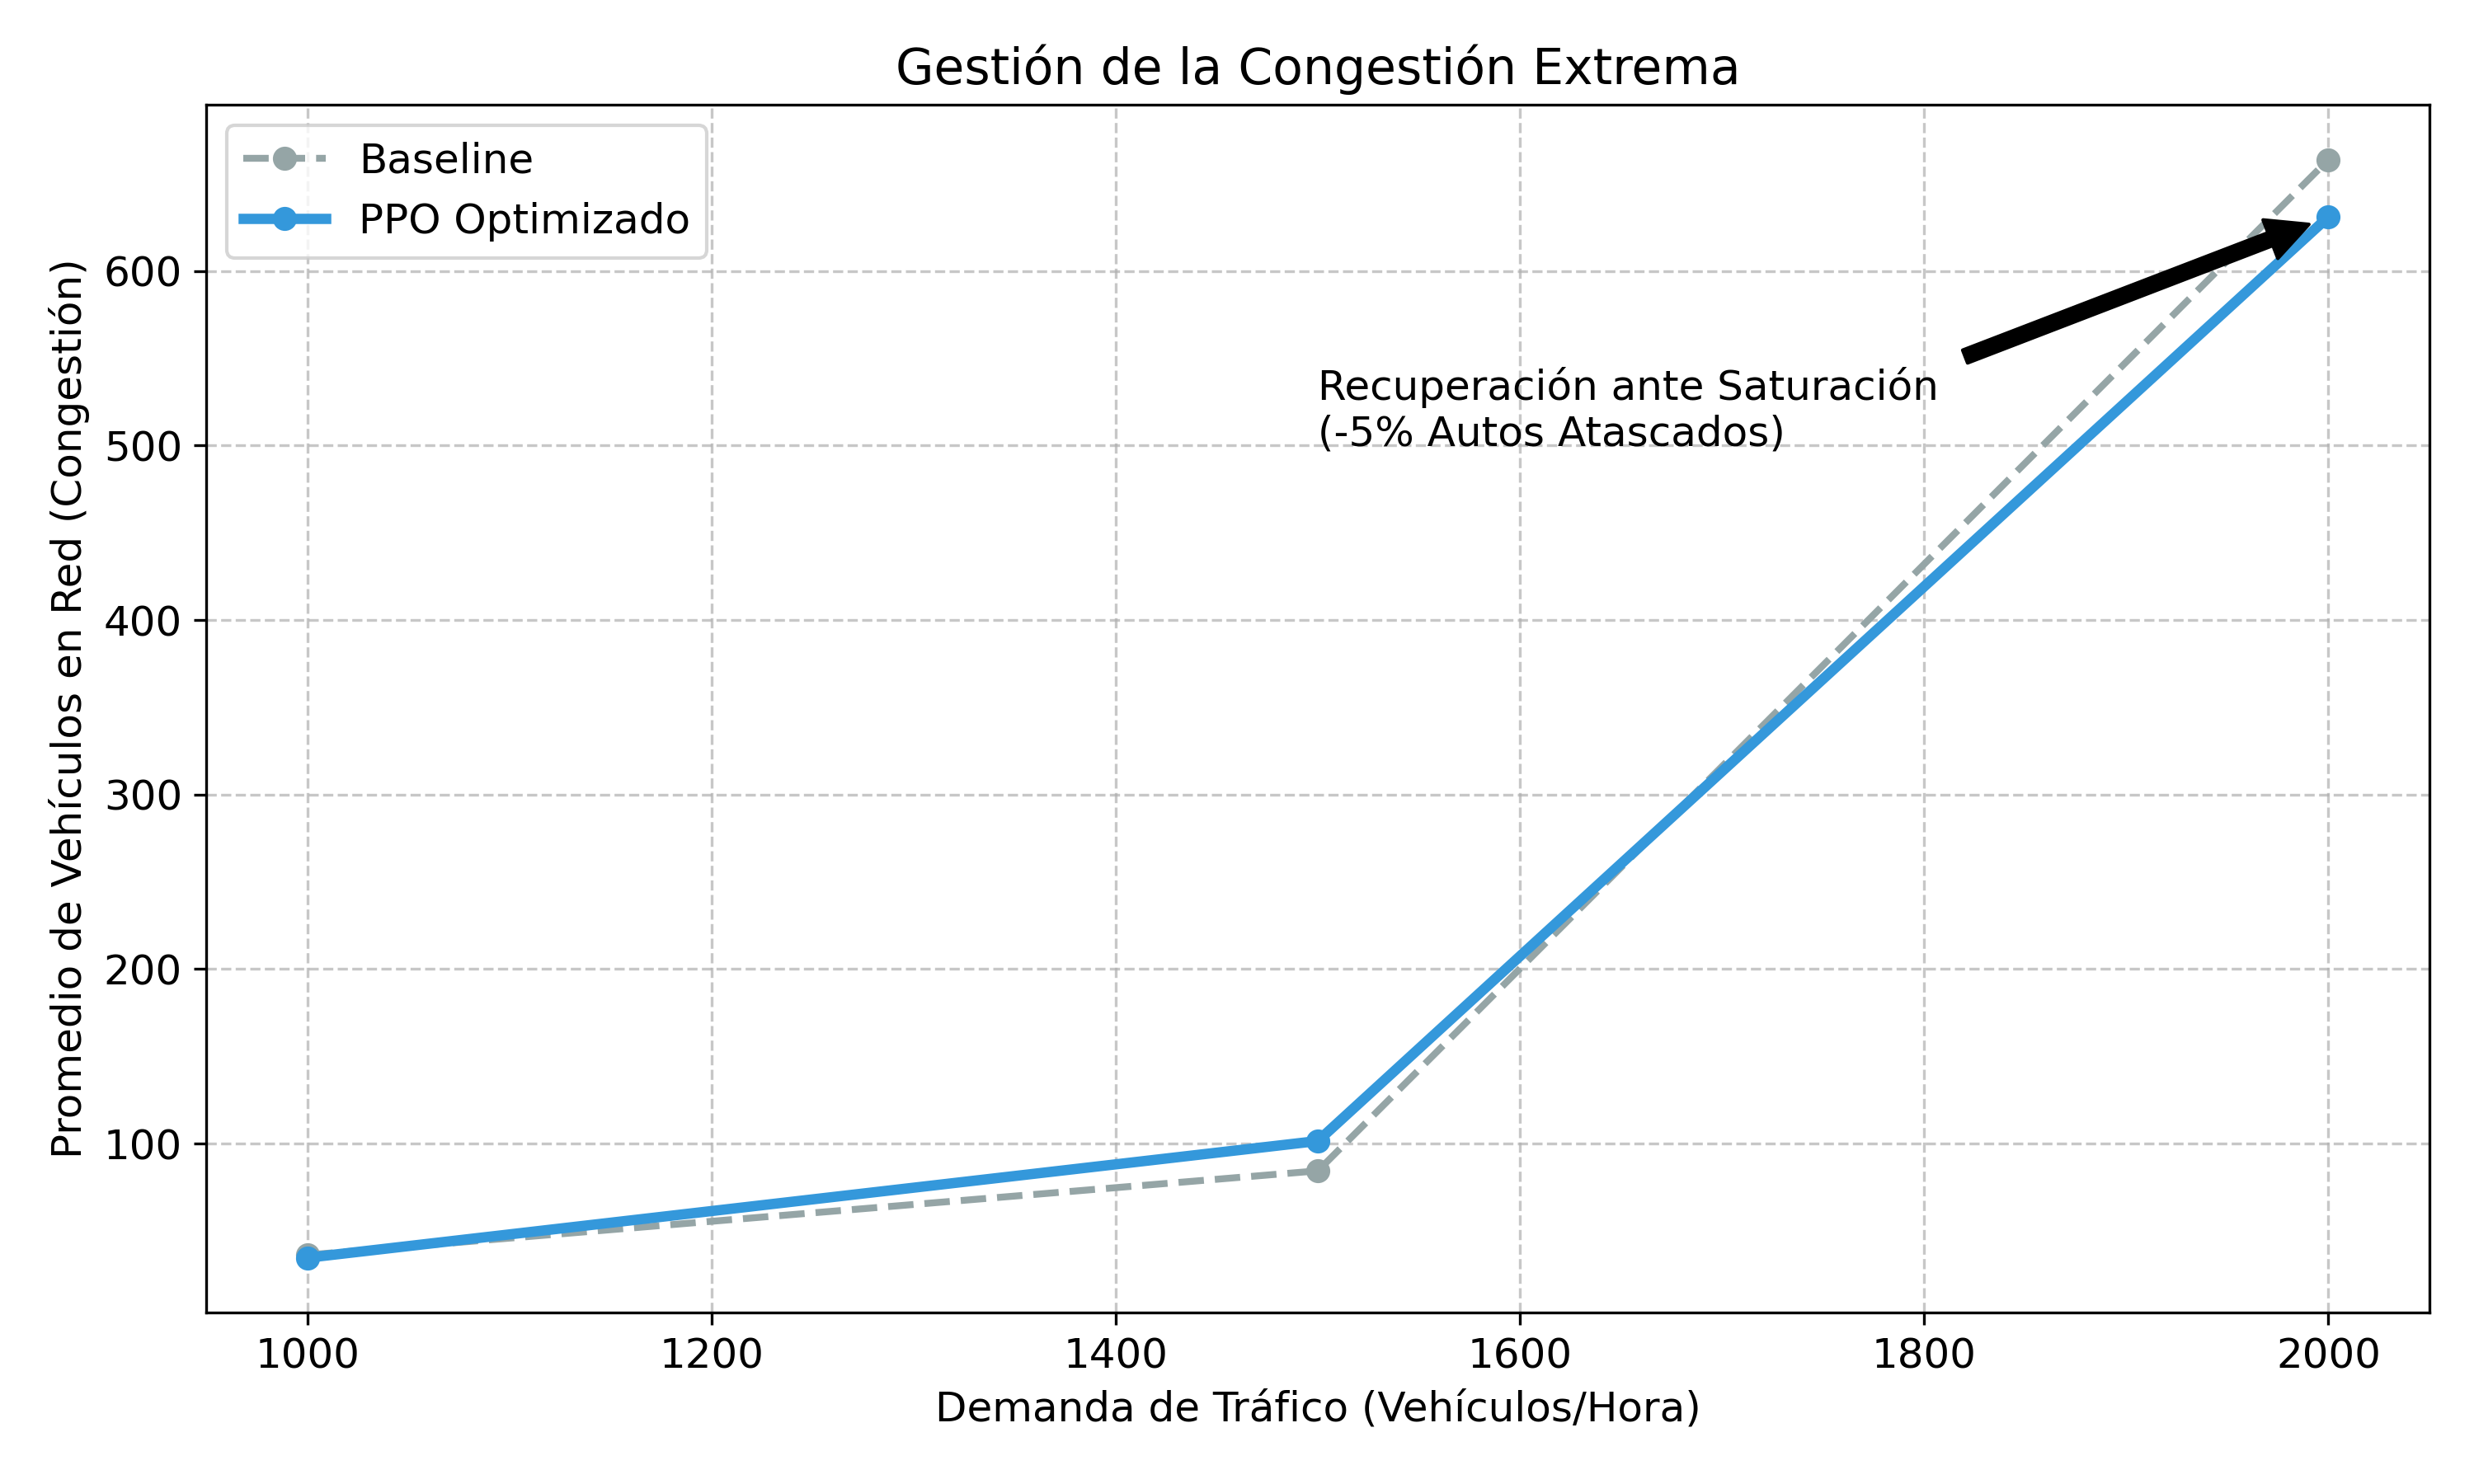
\includegraphics[width=0.8\textwidth]{images/congestion_levels.png}
    \caption{Niveles de congestión (vehículos detenidos) a lo largo del tiempo.}
    \label{fig:congestion_levels}
\end{figure}

El agente mantiene los niveles de congestión controlados, evitando el efecto acumulativo que se observa en el control de tiempo fijo, donde las colas remanentes de un ciclo obstruyen el siguiente.

\section{Análisis de sensibilidad del reward}
Durante el desarrollo, se observó que el diseño de la recompensa es crítico:

\begin{itemize}
    \item \textbf{Sin penalización de desequilibrio ($w_{unbalance}=0$):} El agente tendía a caer en políticas de hold infinito, dejando una fase en rojo durante periodos excesivos si el flujo entrante era constante.
    \item \textbf{Sin costo de cambio ($w_{switch}=0$):} El agente oscilaba rápidamente, lo cual es inseguro.
\end{itemize}
La combinación final de pesos ($w_{queue}=1.0, w_{unbalance}=0.2, w_{switch}=5.0$) logró el equilibrio deseado entre eficiencia y seguridad.



%\chapter{Discussion}
%\label{chap:results}
%\input{chapters/discussion.tex}


\chapter{Conclusiones y Trabajo Futuro}
\label{chap:conclusions}
\section{Conclusiones generales}
El desarrollo de este sistema de control semafórico adaptativo ha permitido validar la hipótesis de que el Deep Reinforcement Learning es una herramienta viable y superior para la gestión del tráfico urbano.

\begin{enumerate}
    \item \textbf{Eficiencia Operativa:} Se logró una reducción del \textbf{60\% en las colas}, lo que impacta directamente en la reducción de tiempos de viaje y consumo de combustible.
    \item \textbf{Adaptabilidad Real:} El agente demostró capacidad para manejar patrones de tráfico asimétricos y ráfagas repentinas, escenarios donde los sistemas tradicionales fallan sistemáticamente.
    \item \textbf{Viabilidad de Implementación:} La inclusión de restricciones de seguridad (\texttt{min\_green}) y penalizaciones por inestabilidad asegura que la política aprendida sea segura y aplicable en el mundo real, no solo una curiosidad teórica.
\end{enumerate}

\section{Limitaciones}
\begin{itemize}
    \item \textbf{Alcance del Modelo:} El estudio se limitó a una intersección aislada. En una red urbana, la coordinación entre múltiples cruces es fundamental y no fue abordada.
    \item \textbf{Percepción Perfecta:} Se asumió que el agente conoce la longitud exacta de la cola. En la realidad, los sensores físicos tienen ruido o fallas, lo que podría afectar el desempeño en campo.
    \item \textbf{Actores Vulnerables:} No se modelaron explícitamente peatones ni ciclistas, cuya seguridad debe ser prioritaria en cualquier implementación real.
\end{itemize}

\section{Propuestas de trabajo futuro}
Para avanzar hacia una implementación en campo, se sugieren las siguientes líneas de investigación:

\begin{itemize}
    \item \textbf{Control Multi-Agente (MARL):} Extender el sistema a un corredor vial utilizando esquemas coordinados entre intersecciones vecinas \cite{marl_chu2020,haps_ppo2025}.
    \item \textbf{Visión por Computador:} Reemplazar los sensores inductivos simulados por un módulo de visión que estime las colas a partir de cámaras de tráfico reales.
    \item \textbf{Observación Parcial y Robustez:} Evaluar el desempeño del agente bajo ruido, pérdida de sensores o estados parcialmente observables para medir su tolerancia a incertidumbre \cite{robust_tan2020}.
    \item \textbf{Vehículos Conectados (V2X):} Integrar información de vehículos conectados para mejorar la estimación del estado y permitir una gestión más anticipada del tráfico \cite{connected_long2022}.
\end{itemize}





%%%%%%% Bibliography %%%%%%%%
%\bibliographystyle{bst/IEEEtran} 
%\bibliography{bib/IEEEreferences} 
\begin{thebibliography}{99}

\bibitem{survey_prajapati2024}
M. Prajapati, A. K. Upadhyay, H. Patil, and J. Dongradive, ``A Review of Deep Reinforcement Learning for Traffic Signal Control,'' \textit{International Journal for Multidisciplinary Research}, 2024, doi: \url{https://doi.org/10.36948/ijfmr.2024.v06i01.11650}.

\bibitem{survey_haydari2022}
A. Haydari and Y. Yilmaz, ``Deep Reinforcement Learning for Intelligent Transportation Systems: A Survey,'' \textit{IEEE Transactions on Intelligent Transportation Systems}, 2022, doi: \url{https://doi.org/10.1109/TITS.2020.3008612}.

\bibitem{review_noaeen2022}
M. Noaeen, A. Naik, L. Goodman, J. Crebo, T. Abrar, Z. S. H. Abad, A. L. Bazzan, and B. Far, ``Reinforcement Learning in Urban Network Traffic Signal Control: A Systematic Literature Review,'' \textit{Expert Systems with Applications}, 2022, doi: \url{https://doi.org/10.1016/j.eswa.2022.116830}.

\bibitem{review_rasheed2020}
F. Rasheed, K. A. Yau, R. M. Noor, C. Wu, and Y. Low, ``Deep Reinforcement Learning for Traffic Signal Control: A Review,'' \textit{IEEE Access}, 2020, doi: \url{https://doi.org/10.1109/ACCESS.2020.3034141}.

\bibitem{benchmark_ault2021}
J. Ault and G. Sharon, ``Reinforcement Learning Benchmarks for Traffic Signal Control,'' \textit{Proceedings of NeurIPS Track on Datasets and Benchmarks}, 2021. Available: \url{https://openreview.net/forum?id=a61Bq-B20b}.

\bibitem{case_gokulan2020}
B. P. Gokulan and A. Srinivasan, ``Traffic Signal Control Using Deep Reinforcement Learning: A Case Study,'' 2020. Available: \url{https://doi.org/10.48550/arXiv.2107.01347}.

\bibitem{rl_sutton2018}
R. S. Sutton and A. G. Barto, \textit{Reinforcement Learning: An Introduction}. 2018. ISBN: 9780262039246.

\bibitem{compare_ouyang2024}
C. Ouyang, Z. Zhan, and F. Lv, ``A Comparative Study of Traffic Signal Control Based on Reinforcement Learning Algorithms,'' \textit{World Electric Vehicle Journal}, 2024, doi: \url{https://doi.org/10.3390/wevj15060246}.

\bibitem{ppo_karedla2025}
G. S. H. Karedla, A. Satapathy, A. H. Shaik, and S. S. Nallagondla, ``Optimizing Urban Traffic Flow with Adaptive Signal Updates Using Proximal Policy Optimization Algorithm,'' 2025, doi: \url{https://doi.org/10.1109/ICACT67549.2025.11351470}.

\bibitem{haps_ppo2025}
Q. Lu, H. Fang, Z. Yin, and G. Zhu, ``HAPS-PPO: A Multi-Agent Reinforcement Learning Architecture for Coordinated Regional Control of Traffic Signals in Heterogeneous Road Networks,'' \textit{Applied Sciences}, 2025, doi: \url{https://doi.org/10.3390/app152010945}.

\bibitem{survey_zhao2024}
H. Zhao, C. Dong, J. Cao, and Q. Chen, ``A Survey on Deep Reinforcement Learning Approaches for Traffic Signal Control,'' \textit{Engineering Applications of Artificial Intelligence}, 2024, doi: \url{https://doi.org/10.1016/j.engappai.2024.108100}.

\bibitem{liang2019}
X. Liang, X. Du, G. Wang, and Z. Han, ``A Deep Reinforcement Learning Network for Traffic Light Cycle Control,'' \textit{IEEE Transactions on Vehicular Technology}, 2019, doi: \url{https://doi.org/10.1109/TVT.2018.2890726}.

\bibitem{colight2019}
H. Wei, N. Xu, H. Zhang, G. Zheng, X. Zang, C. Chen, W. Zhang, Y. Zhu, K. Xu, and Z. Li, ``CoLight,'' \textit{Proceedings of the 28th ACM International Conference on Information and Knowledge Management}, 2019, doi: \url{https://doi.org/10.1145/3357384.3357902}.

\bibitem{metalight2020}
X. Zang, H. Yao, G. Zheng, N. Xu, K. Xu, and Z. Li, ``MetaLight: Value-Based Meta-Reinforcement Learning for Traffic Signal Control,'' \textit{Proceedings of the AAAI Conference on Artificial Intelligence}, 2020, doi: \url{https://doi.org/10.1609/aaai.v34i01.5467}.

\bibitem{marl_chu2020}
T. Chu, J. Wang, L. Codeca, and Z. Li, ``Multi-Agent Deep Reinforcement Learning for Large-Scale Traffic Signal Control,'' \textit{IEEE Transactions on Intelligent Transportation Systems}, 2020, doi: \url{https://doi.org/10.1109/TITS.2019.2901791}.

\bibitem{networkwide_li2021}
Z. Li, H. Yu, G. Zhang, S. Dong, and C. Xu, ``Network-Wide Traffic Signal Control Optimization Using a Multi-Agent Deep Reinforcement Learning,'' \textit{Transportation Research Part C}, 2021, doi: \url{https://doi.org/10.1016/j.trc.2021.103059}.

\bibitem{attendlight2020}
A. Oroojlooy, M. Nazari, D. Hajinezhad, and J. Silva, ``AttendLight: Universal Attention-Based Reinforcement Learning Model for Traffic Signal Control,'' 2020. Available: \url{https://arxiv.org/abs/2010.05772}.

\bibitem{robust_tan2020}
K. L. Tan, A. Sharma, and S. Sarkar, ``Robust Deep Reinforcement Learning for Traffic Signal Control,'' \textit{Journal of Big Data Analytics in Transportation}, 2020, doi: \url{https://doi.org/10.1007/s42421-020-00029-6}.

\bibitem{connected_long2022}
M. Long, X. Zou, Y. Zhou, and E. Chung, ``Deep Reinforcement Learning for Transit Signal Priority in a Connected Environment,'' \textit{Transportation Research Part C}, 2022, doi: \url{https://doi.org/10.1016/j.trc.2022.103814}.

\bibitem{roleaware_zhang2025}
R. Zhang, ``Role-Aware Multi-Agent Reinforcement Learning for Coordinated Emergency Traffic Control,'' NeurIPS 2025. Available: \url{https://openreview.net/forum?id=Role-aware-MARL}.

\bibitem{presslight2019}
H. Wei, C. Chen, G. Zheng, K. Wu, V. Gayah, K. Xu, and Z. Li, ``PressLight,'' 2019, doi: \url{https://doi.org/10.1145/3292500.3330949}.

\bibitem{stable_baselines3_2021}
A. Raffin, A. Hill, A. Gleave, A. Kanervisto, M. Ernestus, and N. Dormann, ``Stable-Baselines3: Reliable Reinforcement Learning Implementations,'' \textit{Journal of Machine Learning Research}, 2021. Available: \url{http://jmlr.org/papers/v22/20-1364.html}.

\bibitem{gymnasium_2023}
M. Towers et al., ``Gymnasium,'' 2023, doi: \url{https://doi.org/10.5281/zenodo.8127026}.

\bibitem{optuna_2019}
T. Akiba, S. Sano, T. Yanase, T. Ohta, and M. Koyama, ``Optuna,'' \textit{Proceedings of the 25th ACM SIGKDD International Conference on Knowledge Discovery \& Data Mining}, 2019, doi: \url{https://doi.org/10.1145/3292500.3330701}.

\bibitem{excel_7_eltantawy2010}
S. El-Tantawy and B. Abdulhai, ``An Agent-Based Learning Towards Decentralized and Coordinated Traffic Signal Control,'' \textit{13th International IEEE Conference on Intelligent Transportation Systems}, 2010, doi: \url{https://doi.org/10.1109/ITSC.2010.5625066}.

\bibitem{excel_8_zhu2019}
L. Zhu, F. R. Yu, Y. Wang, B. Ning, and T. Tang, ``Big Data Analytics in Intelligent Transportation Systems: A Survey,'' \textit{IEEE Transactions on Intelligent Transportation Systems}, 2019, doi: \url{https://doi.org/10.1109/TITS.2018.2815678}.

\bibitem{excel_9_chen2020}
C. Chen, H. Wei, N. Xu, G. Zheng, M. Yang, Y. Xiong, K. Xu, and Z. Li, ``Toward A Thousand Lights: Decentralized Deep Reinforcement Learning for Large-Scale Traffic Signal Control,'' \textit{Proceedings of the AAAI Conference on Artificial Intelligence}, 2020, doi: \url{https://doi.org/10.1609/aaai.v34i04.5744}.

\bibitem{excel_13_kadioglu2024}
S. Kadioglu and B. Kleynhans, ``Building Higher-Order Abstractions from the Components of Recommender Systems,'' \textit{Proceedings of the AAAI Conference on Artificial Intelligence}, 2024, doi: \url{https://doi.org/10.1609/aaai.v38i21.30341}.

\bibitem{excel_16_xu2024}
C. Xu, H. Wang, W. Wang, P. Zheng, and H. Chen, ``Geometric-Facilitated Denoising Diffusion Model for 3D Molecule Generation,'' \textit{Proceedings of the AAAI Conference on Artificial Intelligence}, 2024. Available: \url{https://ojs.aaai.org/index.php/AAAI/article/view/27787}.

\bibitem{excel_18_hu2022}
X. Hu, Z. Zheng, D. Chen, X. Zhang, and J. Sun, ``Processing, Assessing, and Enhancing the Waymo Autonomous Vehicle Open Dataset for Driving Behavior Research,'' \textit{Transportation Research Part C: Emerging Technologies}, 2022, doi: \url{https://doi.org/10.1016/j.trc.2021.103490}.

\bibitem{excel_22_wang2021}
X. Wang, L. Ke, Z. Qiao, and X. Chai, ``Large-Scale Traffic Signal Control Using a Novel Multiagent Reinforcement Learning,'' \textit{IEEE Transactions on Cybernetics}, 2021, doi: \url{https://doi.org/10.1109/TCYB.2020.3015811}.

\bibitem{excel_23_shabestary2018}
S. M. A. Shabestary and B. Abdulhai, ``Deep Learning vs. Discrete Reinforcement Learning for Adaptive Traffic Signal Control,'' \textit{2018 21st International Conference on Intelligent Transportation Systems (ITSC)}, 2018, doi: \url{https://doi.org/10.1109/ITSC.2018.8569549}.

\bibitem{excel_24_khattak2020}
Z. H. Khattak, B. L. Smith, H. Park, and M. D. Fontaine, ``Cooperative Lane Control Application for Fully Connected and Automated Vehicles at Multilane Freeways,'' \textit{Transportation Research Part C: Emerging Technologies}, 2020, doi: \url{https://doi.org/10.1016/j.trc.2019.11.007}.

\bibitem{excel_30_ma2026}
L. Ma, Y. Liu, Y. Liu, C. Ma, and S. Wang, ``Coordinated Multi-Intersection Traffic Signal Control Using a Policy-Regulated Deep Q-Network,'' \textit{Sustainability}, 2026, doi: \url{https://doi.org/10.3390/su18031510}.

\bibitem{excel_32_crielaard2018}
L. Crielaard and P. Papapetrou, ``Explainable Predictions of Adverse Drug Events from Electronic Health Records Via Oracle Coaching,'' \textit{2018 IEEE International Conference on Data Mining Workshops (ICDMW)}, 2018, doi: \url{https://doi.org/10.1109/ICDMW.2018.00108}.

\bibitem{excel_33_he2020}
Z. He, Z. Dong, G. Fang, J. D. Ho, C. Cheung, H. Chang, C. C. Chong, J. Y. Chan, D. T. M. Chan, and K. Kwok, ``Design of a Percutaneous MRI-Guided Needle Robot With Soft Fluid-Driven Actuator,'' \textit{IEEE Robotics and Automation Letters}, 2020, doi: \url{https://doi.org/10.1109/LRA.2020.2969929}.

\bibitem{excel_34_zhang2021}
J. Zhang, F. Y. Wang, and K. Wang, ``Data-Driven Intelligent Transportation Systems: A Survey,'' \textit{IEEE Transactions on Intelligent Transportation Systems}, 2021, doi: \url{https://doi.org/10.1109/TITS.2011.2174862}.

\bibitem{excel_36_tang2024}
D. Tang and Y. Duan, ``Traffic Signal Control Optimization Based on Neural Network in the Framework of Model Predictive Control,'' \textit{Actuators}, 2024, doi: \url{https://doi.org/10.3390/act13070251}.

\bibitem{excel_38_ashwini2025}
Ashwini S. R. and Vidyashankar M., ``Deep Reinforcement Learning for Smart Traffic Control,'' \textit{International Journal of Integrative Studies (IJIS)}, 2025, doi: \url{https://doi.org/10.63856/k40j4b08}.

\end{thebibliography}

%%%%%%% Bibliography %%%%%%%%    

\appendix  
\clearpage % o \cleardoublepage
\addappheadtotoc 
\appendixpage 

\chapter{Anexos}

\section{Repositorio de Código}

El código fuente completo de este proyecto, incluyendo los scripts de entrenamiento, evaluación y configuración de escenarios en SUMO, se encuentra disponible en el siguiente repositorio de GitHub:

\url{https://github.com/Bryansnear/DRLtrafficligth}

\section{Estructura del Proyecto}
\begin{itemize}
    \item \texttt{src/}: Código fuente del agente PPO y el entorno Gym.
    \item \texttt{configs/}: Archivos de configuración YAML.
    \item \texttt{scripts/}: Scripts de ejecución y análisis.
\end{itemize}



\end{document}
